% Options for packages loaded elsewhere
\PassOptionsToPackage{unicode}{hyperref}
\PassOptionsToPackage{hyphens}{url}
%
\documentclass[
  letterpaper,
]{book}

\usepackage{amsmath,amssymb}
\usepackage{lmodern}
\usepackage{iftex}
\ifPDFTeX
  \usepackage[T1]{fontenc}
  \usepackage[utf8]{inputenc}
  \usepackage{textcomp} % provide euro and other symbols
\else % if luatex or xetex
  \usepackage{unicode-math}
  \defaultfontfeatures{Scale=MatchLowercase}
  \defaultfontfeatures[\rmfamily]{Ligatures=TeX,Scale=1}
\fi
% Use upquote if available, for straight quotes in verbatim environments
\IfFileExists{upquote.sty}{\usepackage{upquote}}{}
\IfFileExists{microtype.sty}{% use microtype if available
  \usepackage[]{microtype}
  \UseMicrotypeSet[protrusion]{basicmath} % disable protrusion for tt fonts
}{}
\makeatletter
\@ifundefined{KOMAClassName}{% if non-KOMA class
  \IfFileExists{parskip.sty}{%
    \usepackage{parskip}
  }{% else
    \setlength{\parindent}{0pt}
    \setlength{\parskip}{6pt plus 2pt minus 1pt}}
}{% if KOMA class
  \KOMAoptions{parskip=half}}
\makeatother
\usepackage{xcolor}
\setlength{\emergencystretch}{3em} % prevent overfull lines
\setcounter{secnumdepth}{5}
% Make \paragraph and \subparagraph free-standing
\ifx\paragraph\undefined\else
  \let\oldparagraph\paragraph
  \renewcommand{\paragraph}[1]{\oldparagraph{#1}\mbox{}}
\fi
\ifx\subparagraph\undefined\else
  \let\oldsubparagraph\subparagraph
  \renewcommand{\subparagraph}[1]{\oldsubparagraph{#1}\mbox{}}
\fi

\usepackage{color}
\usepackage{fancyvrb}
\newcommand{\VerbBar}{|}
\newcommand{\VERB}{\Verb[commandchars=\\\{\}]}
\DefineVerbatimEnvironment{Highlighting}{Verbatim}{commandchars=\\\{\}}
% Add ',fontsize=\small' for more characters per line
\usepackage{framed}
\definecolor{shadecolor}{RGB}{241,243,245}
\newenvironment{Shaded}{\begin{snugshade}}{\end{snugshade}}
\newcommand{\AlertTok}[1]{\textcolor[rgb]{0.68,0.00,0.00}{#1}}
\newcommand{\AnnotationTok}[1]{\textcolor[rgb]{0.37,0.37,0.37}{#1}}
\newcommand{\AttributeTok}[1]{\textcolor[rgb]{0.40,0.45,0.13}{#1}}
\newcommand{\BaseNTok}[1]{\textcolor[rgb]{0.68,0.00,0.00}{#1}}
\newcommand{\BuiltInTok}[1]{\textcolor[rgb]{0.00,0.23,0.31}{#1}}
\newcommand{\CharTok}[1]{\textcolor[rgb]{0.13,0.47,0.30}{#1}}
\newcommand{\CommentTok}[1]{\textcolor[rgb]{0.37,0.37,0.37}{#1}}
\newcommand{\CommentVarTok}[1]{\textcolor[rgb]{0.37,0.37,0.37}{\textit{#1}}}
\newcommand{\ConstantTok}[1]{\textcolor[rgb]{0.56,0.35,0.01}{#1}}
\newcommand{\ControlFlowTok}[1]{\textcolor[rgb]{0.00,0.23,0.31}{#1}}
\newcommand{\DataTypeTok}[1]{\textcolor[rgb]{0.68,0.00,0.00}{#1}}
\newcommand{\DecValTok}[1]{\textcolor[rgb]{0.68,0.00,0.00}{#1}}
\newcommand{\DocumentationTok}[1]{\textcolor[rgb]{0.37,0.37,0.37}{\textit{#1}}}
\newcommand{\ErrorTok}[1]{\textcolor[rgb]{0.68,0.00,0.00}{#1}}
\newcommand{\ExtensionTok}[1]{\textcolor[rgb]{0.00,0.23,0.31}{#1}}
\newcommand{\FloatTok}[1]{\textcolor[rgb]{0.68,0.00,0.00}{#1}}
\newcommand{\FunctionTok}[1]{\textcolor[rgb]{0.28,0.35,0.67}{#1}}
\newcommand{\ImportTok}[1]{\textcolor[rgb]{0.00,0.46,0.62}{#1}}
\newcommand{\InformationTok}[1]{\textcolor[rgb]{0.37,0.37,0.37}{#1}}
\newcommand{\KeywordTok}[1]{\textcolor[rgb]{0.00,0.23,0.31}{#1}}
\newcommand{\NormalTok}[1]{\textcolor[rgb]{0.00,0.23,0.31}{#1}}
\newcommand{\OperatorTok}[1]{\textcolor[rgb]{0.37,0.37,0.37}{#1}}
\newcommand{\OtherTok}[1]{\textcolor[rgb]{0.00,0.23,0.31}{#1}}
\newcommand{\PreprocessorTok}[1]{\textcolor[rgb]{0.68,0.00,0.00}{#1}}
\newcommand{\RegionMarkerTok}[1]{\textcolor[rgb]{0.00,0.23,0.31}{#1}}
\newcommand{\SpecialCharTok}[1]{\textcolor[rgb]{0.37,0.37,0.37}{#1}}
\newcommand{\SpecialStringTok}[1]{\textcolor[rgb]{0.13,0.47,0.30}{#1}}
\newcommand{\StringTok}[1]{\textcolor[rgb]{0.13,0.47,0.30}{#1}}
\newcommand{\VariableTok}[1]{\textcolor[rgb]{0.07,0.07,0.07}{#1}}
\newcommand{\VerbatimStringTok}[1]{\textcolor[rgb]{0.13,0.47,0.30}{#1}}
\newcommand{\WarningTok}[1]{\textcolor[rgb]{0.37,0.37,0.37}{\textit{#1}}}

\providecommand{\tightlist}{%
  \setlength{\itemsep}{0pt}\setlength{\parskip}{0pt}}\usepackage{longtable,booktabs,array}
\usepackage{calc} % for calculating minipage widths
% Correct order of tables after \paragraph or \subparagraph
\usepackage{etoolbox}
\makeatletter
\patchcmd\longtable{\par}{\if@noskipsec\mbox{}\fi\par}{}{}
\makeatother
% Allow footnotes in longtable head/foot
\IfFileExists{footnotehyper.sty}{\usepackage{footnotehyper}}{\usepackage{footnote}}
\makesavenoteenv{longtable}
\usepackage{graphicx}
\makeatletter
\def\maxwidth{\ifdim\Gin@nat@width>\linewidth\linewidth\else\Gin@nat@width\fi}
\def\maxheight{\ifdim\Gin@nat@height>\textheight\textheight\else\Gin@nat@height\fi}
\makeatother
% Scale images if necessary, so that they will not overflow the page
% margins by default, and it is still possible to overwrite the defaults
% using explicit options in \includegraphics[width, height, ...]{}
\setkeys{Gin}{width=\maxwidth,height=\maxheight,keepaspectratio}
% Set default figure placement to htbp
\makeatletter
\def\fps@figure{htbp}
\makeatother

\usepackage{booktabs}
\usepackage{longtable}
\usepackage{array}
\usepackage{multirow}
\usepackage{wrapfig}
\usepackage{float}
\usepackage{colortbl}
\usepackage{pdflscape}
\usepackage{tabu}
\usepackage{threeparttable}
\usepackage{threeparttablex}
\usepackage[normalem]{ulem}
\usepackage{makecell}
\usepackage{xcolor}
\makeatletter
\@ifpackageloaded{tcolorbox}{}{\usepackage[many]{tcolorbox}}
\@ifpackageloaded{fontawesome5}{}{\usepackage{fontawesome5}}
\definecolor{quarto-callout-color}{HTML}{909090}
\definecolor{quarto-callout-note-color}{HTML}{0758E5}
\definecolor{quarto-callout-important-color}{HTML}{CC1914}
\definecolor{quarto-callout-warning-color}{HTML}{EB9113}
\definecolor{quarto-callout-tip-color}{HTML}{00A047}
\definecolor{quarto-callout-caution-color}{HTML}{FC5300}
\definecolor{quarto-callout-color-frame}{HTML}{acacac}
\definecolor{quarto-callout-note-color-frame}{HTML}{4582ec}
\definecolor{quarto-callout-important-color-frame}{HTML}{d9534f}
\definecolor{quarto-callout-warning-color-frame}{HTML}{f0ad4e}
\definecolor{quarto-callout-tip-color-frame}{HTML}{02b875}
\definecolor{quarto-callout-caution-color-frame}{HTML}{fd7e14}
\makeatother
\makeatletter
\makeatother
\makeatletter
\@ifpackageloaded{bookmark}{}{\usepackage{bookmark}}
\makeatother
\makeatletter
\@ifpackageloaded{caption}{}{\usepackage{caption}}
\AtBeginDocument{%
\ifdefined\contentsname
  \renewcommand*\contentsname{Table of contents}
\else
  \newcommand\contentsname{Table of contents}
\fi
\ifdefined\listfigurename
  \renewcommand*\listfigurename{List of Figures}
\else
  \newcommand\listfigurename{List of Figures}
\fi
\ifdefined\listtablename
  \renewcommand*\listtablename{List of Tables}
\else
  \newcommand\listtablename{List of Tables}
\fi
\ifdefined\figurename
  \renewcommand*\figurename{Figure}
\else
  \newcommand\figurename{Figure}
\fi
\ifdefined\tablename
  \renewcommand*\tablename{Table}
\else
  \newcommand\tablename{Table}
\fi
}
\@ifpackageloaded{float}{}{\usepackage{float}}
\floatstyle{ruled}
\@ifundefined{c@chapter}{\newfloat{codelisting}{h}{lop}}{\newfloat{codelisting}{h}{lop}[chapter]}
\floatname{codelisting}{Listing}
\newcommand*\listoflistings{\listof{codelisting}{List of Listings}}
\makeatother
\makeatletter
\@ifpackageloaded{caption}{}{\usepackage{caption}}
\@ifpackageloaded{subcaption}{}{\usepackage{subcaption}}
\makeatother
\makeatletter
\@ifpackageloaded{tcolorbox}{}{\usepackage[many]{tcolorbox}}
\makeatother
\makeatletter
\@ifundefined{shadecolor}{\definecolor{shadecolor}{rgb}{.97, .97, .97}}
\makeatother
\makeatletter
\makeatother
\ifLuaTeX
  \usepackage{selnolig}  % disable illegal ligatures
\fi
\IfFileExists{bookmark.sty}{\usepackage{bookmark}}{\usepackage{hyperref}}
\IfFileExists{xurl.sty}{\usepackage{xurl}}{} % add URL line breaks if available
\urlstyle{same} % disable monospaced font for URLs
\hypersetup{
  pdftitle={RAP\_WORKSHOP\_BOOK},
  pdfauthor={Data Science Hub},
  hidelinks,
  pdfcreator={LaTeX via pandoc}}

\title{RAP\_WORKSHOP\_BOOK}
\author{Data Science Hub}
\date{16/04/2024}

\begin{document}
\frontmatter
\maketitle
\ifdefined\Shaded\renewenvironment{Shaded}{\begin{tcolorbox}[boxrule=0pt, borderline west={3pt}{0pt}{shadecolor}, breakable, frame hidden, enhanced, interior hidden, sharp corners]}{\end{tcolorbox}}\fi

\renewcommand*\contentsname{Table of contents}
{
\setcounter{tocdepth}{2}
\tableofcontents
}
\mainmatter
\bookmarksetup{startatroot}

\hypertarget{rap-workshop}{%
\chapter{RAP Workshop}\label{rap-workshop}}

Data Science Team\\
2024-04-26

\hfill\break

\begin{tcolorbox}[enhanced jigsaw, arc=.35mm, colbacktitle=quarto-callout-note-color!10!white, toprule=.15mm, titlerule=0mm, opacityback=0, title=\textcolor{quarto-callout-note-color}{\faInfo}\hspace{0.5em}{RAP}, coltitle=black, bottomrule=.15mm, colframe=quarto-callout-note-color-frame, leftrule=.75mm, breakable, opacitybacktitle=0.6, rightrule=.15mm, left=2mm, bottomtitle=1mm, toptitle=1mm, colback=white]
It is important for analysis to be reproducible. Different analysts
using the same methods with the same data should get the same results.
\end{tcolorbox}

RAP is a way of using software engineering techniques to improve the
reproducibility of your analysis. By minimising manual steps, using
version control , and producing good documentation analysis can be
higher quality, reproducible, reuseable and more efficient. Applying RAP
principles helps you comply with the requirements in the
\href{https://www.gov.uk/government/publications/the-aqua-book-guidance-on-producing-quality-analysis-for-government}{AQUA
book} for good quality assurance, and was recommended in the
\href{https://www.gov.uk/government/publications/better-broader-safer-using-health-data-for-research-and-analysis}{Goldacre
Review} into using health data for research and analysis.

The key advantages of RAP are:

\begin{itemize}
\item
  Higher quality analysis and reduced risk, with quality assurance built
  into all parts of the process
\item
  More efficient and reliable processes
\item
  Improved transparency and greater confidence in the analysis from
  producers, managers, and users
\item
  Improved business continuity and knowledge management
\item
  Analysis that is easier to adapt and reuse
\end{itemize}

In DHSC we have a variety of tools to help develop and implement RAPs
into your work. This book aims to familiarise yourself these tools and
fundamentals of RAP.

\hypertarget{what-makes-a-good-rap}{%
\section{What makes a good RAP?}\label{what-makes-a-good-rap}}

\textbf{Code}

The best way to incorporate RAP into your work is using code, and in
particular open source languages such as R or Python.

\begin{itemize}
\item
  Your code will use an appropirate coding standard to ensure
  readability, i.e.~the \href{https://style.tidyverse.org/}{Tidy style
  guide}.
\item
  Your code will require minimal manual intervention to produce it's
  outputs.
\item
  Your code will be modular and repeated processes written as functions
\item
  Your code will be well structured and organised into appropriate
  folders.
\item
  Your code will have undergone the appropriate level of quality
  assurance (QA).
\item
  Your code will be well documented, including a readme document and
  function.
\item
  Your code will include unit testing.
\item
  Your code will be fully packaged for easy distribution.
\end{itemize}

\textbf{Data / Pipeline}

Analysis can use data from a variety of sources, and in a variety of
formats. For your RAP the data needs to come from a relatively stable
source, so as not to need rewriting at every use.

\begin{itemize}
\item
  Your data will be handled in a tidy format.
\item
  Your data will come from a managed source, such as a database.
\item
  Your pipeline will use continuous integration or continuous deployment
  and run tests.
\end{itemize}

\textbf{Documentation}

To be understood and maintained by future users (including yourself!)
your RAP needs to be well documented. This will help with any issues
running the pipeline, both with the code and any methodology.
Documentation is also an important part of keeping a clear audit trail
for your analysis, this is particularity vital for anything business
critical.

\begin{itemize}
\item
  Your code will produce informative and useful logging (for
  troubleshooting, and ensuring your RAP has run correctly.
\item
  Your code will be version controlled using Git.
\item
  You will produce clear documentation for future users, such as
  READMEs.
\item
  Your code will be published in the open.
\item
  Any changes to your RAP will be clearly documented and signposted,
  i.e.~in a changelog.
\end{itemize}

\textbf{Not all RAPs will include all of the above, but we should aspire
to meet as much as possible and appropriate. We will cover the majority
of the above in this book.}

\textbf{RAP is a code agnostic approach, however this book will focus on
RAP using R.} The principles are transferable to other languages, but
the specifics may not be.

\bookmarksetup{startatroot}

\hypertarget{section}{%
\chapter{}\label{section}}

Summary

The aim of this book is to provide a template for using RAP for
analysis.

It gives the necessary steps to ensure your RAP is easily maintained,
updated and understood.

It has been primarliy designed to accompany a workshop going through the
exercises within, but can also be used as reference material to help
build your RAP independently.

Prerequisites

The prerequisites for taking part in the workshop and completeing the
excersises are:

RStuido installed

Git installed

A Github account, and being a member of the DHSC organisaion on Github

DHSC RAP Template {[}link to chapter{]}

Version Control {[}link to chapter{]}

Project Documentation {[}link to chapter{]}

Logging {[}link to chapter{]}

Inline Documentation {[}link to chapter{]}

Downloading Data {[}link to chapter{]}

Analysis and Output {[}link to chapter{]}

QA {[}link to chapter{]}

Further Links

NHSE RAP Community of Practice

DHSCTools

Analysis Function RAP strategy

AQUA Book

Duck Book

Goldacre Review

NHSE Health RAP Playbook

\bookmarksetup{startatroot}

\hypertarget{dhsc-rap-template}{%
\chapter{DHSC RAP Template}\label{dhsc-rap-template}}

\begin{tcolorbox}[enhanced jigsaw, arc=.35mm, colbacktitle=quarto-callout-note-color!10!white, toprule=.15mm, titlerule=0mm, opacityback=0, title=\textcolor{quarto-callout-note-color}{\faInfo}\hspace{0.5em}{Key Points}, coltitle=black, bottomrule=.15mm, colframe=quarto-callout-note-color-frame, leftrule=.75mm, breakable, opacitybacktitle=0.6, rightrule=.15mm, left=2mm, bottomtitle=1mm, toptitle=1mm, colback=white]

\begin{itemize}
\item
  The DHSC RAP template provides you with the basic file structure for
  you RAP
\item
  The template provides a series of useful files to remove some the
  intial overhead when starting a new project.
\item
  The RAP template can be accessed through the
  \texttt{DataS-DHSC/DHSCtools} package hosted on Github.
\end{itemize}

\end{tcolorbox}

The first step to producing your RAP is creating an R project in
RStudio. An R project makes it easy to move your work between different
directories without having to change absolute file paths. In DHSC we
have developed a project template that can be used instead of the
standard version, and provides extra features.

The DHSC project template is intended to embed a standard approach to R
programming at DHSC and adheres to coding best practice as set out by
the
\href{https://best-practice-and-impact.github.io/qa-of-code-guidance/}{UK
Government Analytical Community - Quality assurance of code for analysis
and research}.

The template creates a project structure that closely follows that
enforced by R packages. This allows the use of automated features such
as documenting and unit testing of code as well as simplifying the
process of converting code to a package if needed.

The template gives you the basic file structure for your RAP, along with
a variety of files that will be useful as you develop your pipeline.
This removes some of the overhead in having to create these yourselves,
and acts a reminder to include elements of best practice.

The next section will give a more in depth look at what is contained in
the template. If you just want to know how to install it,
\protect\hyperlink{download}{click here}.

\bookmarksetup{startatroot}

\hypertarget{template-structure}{%
\chapter{Template Structure}\label{template-structure}}

The aim is to write your code in a way to make it reproducible and easy
to follow, with a consistent folder structure across different projects.

The template contains several folders.

\begin{itemize}
\item
  The central project folder, with your key files.
\item
  An R folder in which to store the scripts containing the analysis
  functions.

  An input folder in which to store your data and any input parameters.
\item
  An output folder in which you save your RAP outputs.
\end{itemize}

The template provides a series of useful files to help you build your
RAP. The key ones we'll cover in this book are:

\begin{itemize}
\item
  \texttt{main.r} - This is the script from which you will run your
  code, initialise your packages, and start your logging
\item
  \texttt{.Rproj} - This is an RStudio project file, which helps keep
  your RAP self contained, and avoids the need for absolute file paths
  which are not transferable between different users.
\item
  \texttt{README.Rmd} - This is a document in which you will explain
  your project, how it works and how to run in.
\item
  \texttt{.gitignore} - While version control is essential, not all
  files can be shared. The gitignore files allows you to specify which
  files will not be pushed into a remote repo.
\item
  \texttt{config.yml} - A config file allows you to change parameters
  without needing to edit the code itself. It is written in YAML, a
  simple structured data language.
\end{itemize}

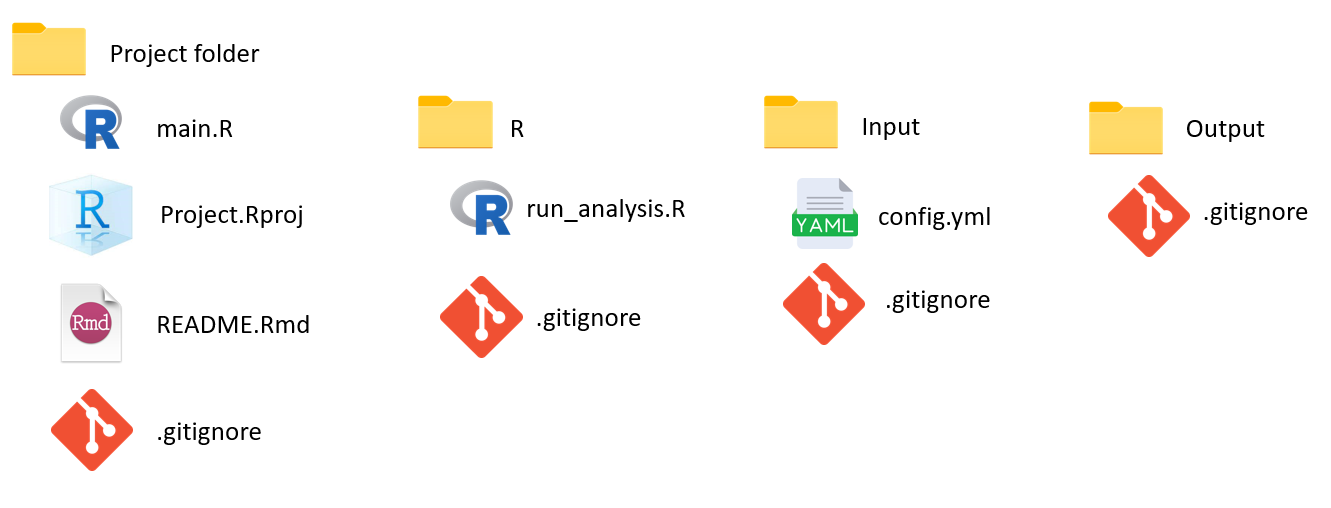
\includegraphics{./images/template_files.PNG}

\hypertarget{using-the-template---best-practice}{%
\section{Using the template - Best
practice}\label{using-the-template---best-practice}}

Use the \texttt{main.R} script to source and call the main function used
to run your analysis and set up your environment, logging, and
dependencies (using the \texttt{librarian} package). Using a standard
entry point to running the analysis will help others understand and run
your code more quickly and also enforces the use of modular functions.

All other scripts should be saved in the \texttt{./R} folder with code
structured into separate files containing logically grouped functions.
For non-packaged projects, please add a section to the start of each
file that explicitly loads all dependencies (either using the
\texttt{library} and \texttt{source} function for smaller projects or
the \texttt{box} and \texttt{renv} packages for larger projects).

Store input parameters and settings in the \texttt{./input/config.yml}
YAML file and sensitive parameters in the \texttt{.REnviron} file (this
file is not version controlled by default in the template).

Store input data and settings in the \texttt{./input} folder and write
any output from the analysis to the \texttt{./output} folder. These
folders contain \texttt{.gitignore} files which prevent their contents
from being version controlled (with the exception of
\texttt{./input/config.yml}).

For small projects, we recommend using the \texttt{librarian} package
and base R \texttt{source} function to manage dependencies; for larger
projects we would recommend using the \texttt{renv} and \texttt{box}
packages for dependency management as well as considering packaging the
project itself on GitHub.

\bookmarksetup{startatroot}

\hypertarget{installing-the-dhsctools-package}{%
\chapter{Installing the DHSCtools
package}\label{installing-the-dhsctools-package}}

There are two packages required for this exercise. The first is
\texttt{devtools}. If you do not have it installed, it can be installed
like a typical package using the following command:

\begin{verbatim}
install.packages("devtools")
\end{verbatim}

You will then need to load the library:

\begin{verbatim}
library(devtools)
\end{verbatim}

The second package required is the DHSC-developed tools package, which
will need to be installed from GitHub. When installing packages from
GitHub, you need to remember to include both the author and the name of
the package. In this case, the author is \texttt{DataS-DHSC}, and the
name of the package is \texttt{DHSCtools}, like so:

\begin{verbatim}
install_github("DataS-DHSC/DHSCtools")
\end{verbatim}

Make sure for follow any instructions in the console during
installation.

One the package is installed, load the library:

\begin{verbatim}
library(DHSCtools)
\end{verbatim}

\bookmarksetup{startatroot}

\hypertarget{set-up-your-template}{%
\chapter{Set up your Template}\label{set-up-your-template}}

After installing the package, to use the DHSC project template go to
File \textgreater{} New Project\ldots{} then select New Directory
followed by DHSC Project Template. Make sure to untick the ``Include
example code?'' checkbox.

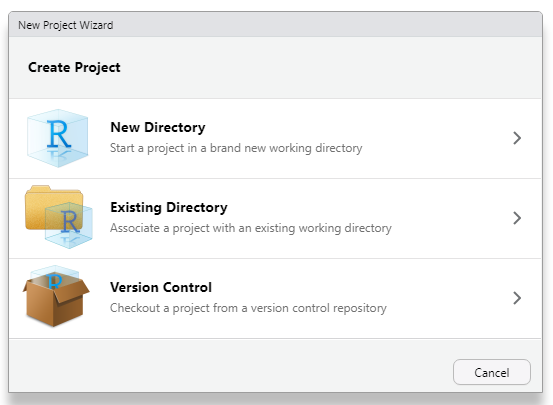
\includegraphics{./images/create_project.PNG}
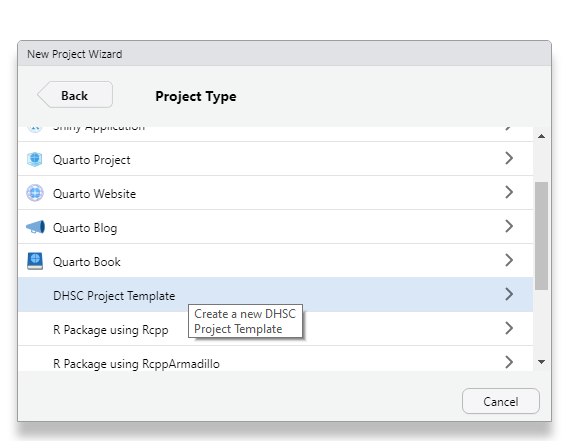
\includegraphics{./images/dhsc project template.PNG}
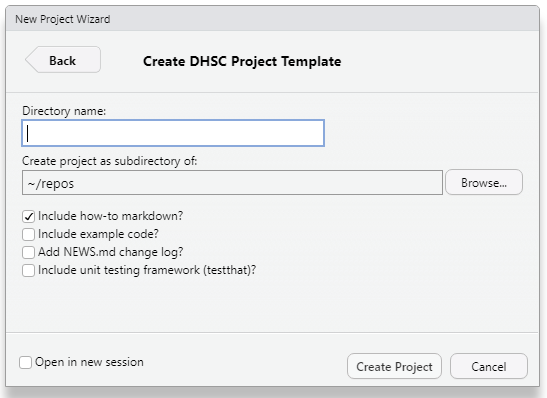
\includegraphics{./images/create_project_2.PNG}

The optional example code contains similar examples to those in this
book, but including them here may cause some confusion later.

\hypertarget{exercise-set-up-your-own-project-template}{%
\section{Exercise: set up your own project
template}\label{exercise-set-up-your-own-project-template}}

In this section, you'll set up a project template of your own. Using any
required steps above, you should:

\begin{enumerate}
\def\labelenumi{\arabic{enumi}.}
\item
  Install the required packages.
\item
  Download the RAP template and create a project.
\end{enumerate}

\bookmarksetup{startatroot}

\hypertarget{version-control-git}{%
\chapter{Version Control \& Git}\label{version-control-git}}

\begin{tcolorbox}[enhanced jigsaw, arc=.35mm, colbacktitle=quarto-callout-note-color!10!white, toprule=.15mm, titlerule=0mm, opacityback=0, title=\textcolor{quarto-callout-note-color}{\faInfo}\hspace{0.5em}{Key Points}, coltitle=black, bottomrule=.15mm, colframe=quarto-callout-note-color-frame, leftrule=.75mm, breakable, opacitybacktitle=0.6, rightrule=.15mm, left=2mm, bottomtitle=1mm, toptitle=1mm, colback=white]

\begin{itemize}
\item
  Version control your RAP using Git
\item
  Use Github to collaborate on your RAP
\item
  Do not push your data or sensitive parameters to Github
\item
  Keep an up to date version of your RAP and your data on Sharepoint.
\end{itemize}

\end{tcolorbox}

\hypertarget{git}{%
\section{Git}\label{git}}

Version control is important to provide an audit trail for your work.
You can see what changes have been made, when, and by who. It also means
that any changes made that end up breaking your RAP can be easily
reversed, and you can revert to a working version.

Git is open source software that handles version control, and is the
most widely used system. It is most commonly used through the command
line, but there a are GUI options available.

Now we have the template for our RAP we should add it to a Git
repository, or repo.

A thorough explanation of Git commands is beyond the scope of this book
but there is a lot of separate training available.
\href{https://education.github.com/git-cheat-sheet-education.pdf}{Here}
is a cheat sheet to give a quick overview of Git commands.

\hypertarget{install-git}{%
\subsection{Install Git}\label{install-git}}

Git is a program available from within the Company Portal in your Start
menu. The software is called `Git For Windows', and will be available in
the `Apps' category. You will need to install this software before
proceeding any further.

\hypertarget{link-git-and-rstudio}{%
\subsection{Link Git and RStudio}\label{link-git-and-rstudio}}

Once you have installed Git, or if you already have it installed, start
by telling RStudio where it can find Git. The first thing you will need
to do is to identify where Git has been installed on your computer. In
the Terminal tab (please note: this is \emph{not} the same as the
Console tab) in RStudio, type the following:

\begin{verbatim}
where git
\end{verbatim}

This should produce the location of the installation of Git on your
machine.

Once you have done this, you will need to:

\begin{itemize}
\tightlist
\item
  Navigate to the \texttt{Tools} menu, and select
  \texttt{Global\ Options}.
\item
  Click on \texttt{Git/SVN}.
\item
  Check \emph{Enable version control interface for Rstudio projects}.
\item
  Set the path to the path given when using the \texttt{where\ git}
  command in the terminal.
\item
  Check \emph{use Git bash as shell for Git projects}.
\end{itemize}

\hypertarget{github}{%
\section{Github}\label{github}}

Github is a web based platform designed to facilitate collaboration when
working on projects version controlled with Git. There are a number of
similar services, some with similar names (i.e.~Gitlab), they share many
similarities, but will have some differing features.

If you do not already have a Github account, now is the time to create
one.

\hypertarget{configure-github-in-rstudio}{%
\subsection{Configure GitHub in
RStudio}\label{configure-github-in-rstudio}}

Github can be linked with RStudio to streamline the version control
process.

First, you now need to tell GitHub who you are. Open Git Shell by
navigating to \texttt{Tools\ \textgreater{}\ Shell} in the RStudio menu.
In the shell, type the following command (replacing ``mygithubusername''
with your actual GitHub username, keeping the quotation marks):

\begin{verbatim}
git config --global user.name "yourgithubusername"
\end{verbatim}

Next, type the following command, including the email address you used
to make your account:

\begin{verbatim}
git config --global user.email "your@email.address"
\end{verbatim}

You can then check the configuration was successful by typing
\texttt{git\ config\ -\/-global\ -\/-list}. It should return something
like the following:

\begin{verbatim}
user.name=yourgithubusername
user.email=your@email.address
\end{verbatim}

You should make a commit of the current version of the project by using
Git\textgreater Commit in RStudio. Make sure to add a comment, such as
``initial commit''.

Now, you can run the snippet of code under the header ``Adding GitHub
support'', which will generate a private Github repository in the DHSC
organisation.

\hypertarget{push-your-project-to-github}{%
\subsection{Push your project to
GitHub}\label{push-your-project-to-github}}

Now that you're set up with Git and RStudio, it's time to push your new
project to GitHub.

Open GitHub in your web browser, and create a new repository. You can do
this as a personal repository, or from within any GitHub organisation to
which you have access (e.g.~DATAS-DHSC). Make sure you give it the exact
same name as your RStudio project, but do \textbf{not} check the
\emph{Initialize this repository with a README} option. Finish this by
clicking the \emph{Create Project} option.

From your GitHub browser window, you will need to copy the two lines of
code from the box labelled \emph{Push an existing repository from the
command line} They may look something like this, depnding on whether it
is a personal or organisation-level repository:

\begin{verbatim}
git remote add origin https://github.com/USERNAME/PROJECT.git
git push -u origin master
\end{verbatim}

Back in RStudio, make sure RStudio is using your new project as the
working directory, and ensure the \texttt{Git} tab is available in the
top right window. (This is the window that also contains the
\texttt{Environment} and \texttt{History} tabs, among others.)

Open \texttt{Tools\ \textgreater{}\ Shell} again, and paste in the two
lines of code you copied from GitHub. Press enter or return to finish.
Your repository, and all its template files, should now be available
within the online repository.

\hypertarget{using-git-and-github-in-dhsc}{%
\section{Using Git and Github in
DHSC}\label{using-git-and-github-in-dhsc}}

It is best practice to do as much of your coding in the open as
possible. However in DHSC we often use sensitive data that cannot be in
the public domain, and some that should not be shared to servers outside
of the DHSC estate. This means that is important to keep data and
sensitive parameters off of Github. This does make sharing your projects
more difficult as these must be stored elsewhere.

The solution to this that we recommend is keeping an up to date version
of your main branch saved on in a shared drive on Sharepoint, along with
your data and parameters. As you make changes, and push them to your
main branch, you should pull these changes into this shared drive. The
team members working on the project can clone the repo from Github, copy
the data from the Sharepoint version into their local repo and do their
work, pushing changes back up to Github.

Files can be prevented from being pushed into a Git rep using a file
called \texttt{.gitingore}. This is a list of files that will not be
pushed with your code. It can refer to specific files, or to all files
with a particular extension.

The template gives you the below \texttt{.gitignore} file.

\begin{verbatim}
# History files.Rhistory`.Rapp.history

# Session Data files
.RData

# User-specific files
.Ruserdata

# Example code in package build process
*-Ex.R

# Output files from R CMD build
*.tar.gz

# Output files from R CMD check
*.Rcheck

# RStudio files
.Rproj.user

# produced vignettes
vignettes/*.html
vignettes/*.pdf

# OAuth2 token, see https://github.com/hadley/httr/releases/tag/v0.3
.httr-oauth

# knitr and R markdown default cache directories
*_cache/
cache/

# Temporary files created by R markdown
*.utf8.md
*.knit.md

# R Environment Variables
.Renviron
.Rproj.user
.Rdata
.DS_Store

# Files added by usethis
docs
\end{verbatim}

\bookmarksetup{startatroot}

\hypertarget{project-documentation---readme-files}{%
\chapter{Project documentation - Readme
files}\label{project-documentation---readme-files}}

\begin{tcolorbox}[enhanced jigsaw, arc=.35mm, colbacktitle=quarto-callout-note-color!10!white, toprule=.15mm, titlerule=0mm, opacityback=0, title=\textcolor{quarto-callout-note-color}{\faInfo}\hspace{0.5em}{Key Points}, coltitle=black, bottomrule=.15mm, colframe=quarto-callout-note-color-frame, leftrule=.75mm, breakable, opacitybacktitle=0.6, rightrule=.15mm, left=2mm, bottomtitle=1mm, toptitle=1mm, colback=white]

\begin{itemize}
\item
  You should include a Readme file for in your RAP explaining what you
  have done, and how the code ca be used.
\item
  You should write your Readme with markdown to help with readability.
\end{itemize}

\end{tcolorbox}

A good Readme file is a key component of reproducible analysis and it
should give users of your analysis/code sufficient information to
understand what it does, and how they can install and run it without
recourse to the project's original author. The Readme file is displayed
on the front page of your github repository.

The
\href{https://www.gov.uk/government/publications/the-aqua-book-guidance-on-producing-quality-analysis-for-government}{Aqua
book} gives guidance on what Readme files should include, which can be
summarised as:

\begin{enumerate}
\def\labelenumi{\arabic{enumi}.}
\item
  Short statement of intent
\item
  Longer description describing the problem that your project solves and
  how it solves it
\item
  Basic installation instructions or link to installation guide
\item
  Example usage
\item
  Screenshot if your project has a graphical user interface (but make
  sure to mask any data if it is not in the public domain)
\item
  Links to related projects
\end{enumerate}

Descriptions of code or data you add to your readme could potentially
get into the public domain and so it is critical you treat readme
descriptions and data examples in the same way you would treat
unpublished data and/or sensitive models.

\hypertarget{project-description}{%
\subsection{Project description}\label{project-description}}

Your Readme should describe what your RAP does, and why you have made
the choices you have.

\begin{itemize}
\item
  Data sources - It should be clear which data you ingest and where you
  take it from. This could be a URL, a file directory, or elsewhere. You
  should also explain the frequency with which you get your data. You
  may choose to describe the data formats in more detail but you might
  also refer or link to a specification document held elsewhere if your
  data or its structure is sensitive in nature.
\item
  Processing/analysis - explain how your code performs the analsysis and
  describe its structure because others may need to change your code. As
  always, we recommend you write modular, loosely coupled code, and so
  it may be useful to include a structure chart explaining how the code
  fits together (see below for a simple example). If you use complex
  models then provide links to the model specification so your users can
  understand how yours calculations are performed (this also allows you
  to restrict access to these specifications).
\item
  Outputs - what are the outputs from this code, who uses them and how?
  If you write to files, then where is this data written to? Again, you
  can refer or link to a specification held elsewhere.
\end{itemize}

\hypertarget{basic-installation-instructions}{%
\subsection{Basic installation
instructions}\label{basic-installation-instructions}}

What does the user need to do to install your code - is it simply a case
of cloning the git repository? It is hoped all package management is
dealt with by the DHSC template (librarian) but are there other tools
your user might need. This is where you specify them and how your users
install them.

\hypertarget{example-usage}{%
\subsection{Example usage}\label{example-usage}}

The default behavior for projects built using the DHSC template is for
you to source the main.R function and for this script to then
orchestrate all subsequent processing. However, you may specify that the
user updates the config.yml file to locate source data and identify
where to write outputs.

\begin{itemize}
\tightlist
\item
  log.txt - progress and errors encountered should all be logged to
  log.txt and so you may wish to tell users what to look for,
  e.g.~particular warning or error messages, messages to say processing
  has finished successfully, etc.
\end{itemize}

\hypertarget{using-markdown-to-describe-your-code}{%
\section{Using markdown to describe your
code}\label{using-markdown-to-describe-your-code}}

The Readme file uses RMarkdown which is a language you can use to add
formatting elements to plain text documents. It is can be very useful
when you want to emphasise or illustrate important aspects of your code
or model.

Use one or more `\#' to create headers, e.g.

\hypertarget{visual}{%
\subsubsection{Visual}\label{visual}}

\hypertarget{header-3}{%
\subsubsection{Header 3}\label{header-3}}

\begin{itemize}
\tightlist
\item
  bullet point

  \begin{itemize}
  \tightlist
  \item
    indented bullet point
  \end{itemize}
\end{itemize}

\begin{enumerate}
\def\labelenumi{\arabic{enumi}.}
\tightlist
\item
  numbered list
\item
  numbered list second item
\end{enumerate}

\hypertarget{table-3.1}{%
\subsubsection{Table 3.1}\label{table-3.1}}

\begin{longtable}[]{@{}ll@{}}
\toprule()
Sharepoint folder & Content category \\
\midrule()
\endhead
input\_data & For data that will need to be preprocessed \\
interim\_data & For compliant data \\
\bottomrule()
\end{longtable}

\hypertarget{image-3.2}{%
\subsubsection{Image 3.2}\label{image-3.2}}

\begin{figure}

{\centering 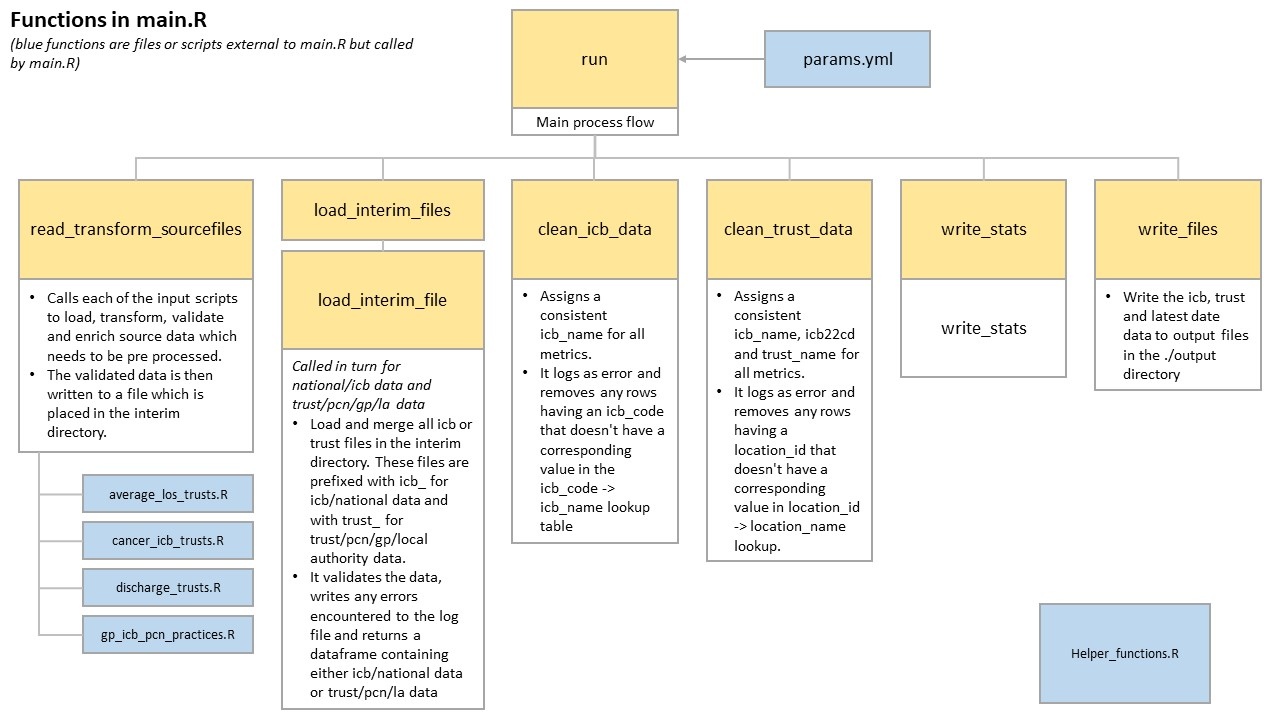
\includegraphics{./images/main_flow.jpg}

}

\caption{Usage}

\end{figure}

\hypertarget{source}{%
\subsubsection{Source}\label{source}}

\texttt{\#\#\#\#\ Header\ 3}

\texttt{-\ \ \ bullet\ point} \texttt{-\ \ \ indented\ bullet\ point}

\texttt{1.\ \ numbered\ list}
\texttt{2.\ \ numbered\ list\ second\ item}

\texttt{\#\#\#\#\ Table\ 3.1}

\texttt{\textbar{}\ Sharepoint\ folder\ \textbar{}\ Content\ category\ \ \ \ \ \ \ \ \ \ \ \ \ \ \ \ \ \ \ \ \ \ \ \ \ \ \ \textbar{}}
\texttt{\textbar{}-\/-\/-\/-\/-\/-\/-\/-\/-\/-\/-\/-\/-\/-\/-\/-\/-\/-\/-\textbar{}:-\/-\/-\/-\/-\/-\/-\/-\/-\/-\/-\/-\/-\/-\/-\/-\/-\/-\/-\/-\/-\/-\/-\/-\/-\/-\/-\/-\/-\/-\/-\/-\/-\/-\/-\/-\/-\/-\/-\/-\/-\/-\/-\textbar{}}
\texttt{\textbar{}\ input\_data\ \ \ \ \ \ \ \ \textbar{}\ For\ data\ that\ will\ need\ to\ be\ preprocessed\ \textbar{}}
\texttt{\textbar{}\ interim\_data\ \ \ \ \ \ \textbar{}\ For\ compliant\ data\ \ \ \ \ \ \ \ \ \ \ \ \ \ \ \ \ \ \ \ \ \ \ \ \ \textbar{}}

\texttt{\#\#\#\#\ Image\ 3.2}

\texttt{!{[}Usage{]}(./main\_flow.jpg)}

\bookmarksetup{startatroot}

\hypertarget{in-line-documentation}{%
\chapter{In line documentation}\label{in-line-documentation}}

\begin{tcolorbox}[enhanced jigsaw, arc=.35mm, colbacktitle=quarto-callout-note-color!10!white, toprule=.15mm, titlerule=0mm, opacityback=0, title=\textcolor{quarto-callout-note-color}{\faInfo}\hspace{0.5em}{Key Points}, coltitle=black, bottomrule=.15mm, colframe=quarto-callout-note-color-frame, leftrule=.75mm, breakable, opacitybacktitle=0.6, rightrule=.15mm, left=2mm, bottomtitle=1mm, toptitle=1mm, colback=white]

\begin{itemize}
\item
  You should comment your code, and keep the comments updated
\item
  Roxygen is a great way to document your functions
\end{itemize}

\end{tcolorbox}

It's important to add comments to your code to help future users
(including yourself) understand how your code works, and why you have
made the decisions you have.

Having documentation in the same place as your code is important as you
cannot guarantee users of your code will read all the other
documentation you have put together, and comments ensure they will know
what your code does.

Your comments don't need to explain what each line does, you should be
writing code in a way that is readable for other users. You should be
describing why you have written things in the way you have if you don't
think it will be obvious.

It's important to keep comments up to date as you refactor your code.
Comments that were once useful will become actively unhelpful if they do
not match the code they are with.

\hypertarget{roxygen2}{%
\section{Roxygen2}\label{roxygen2}}

As discussed in earlier chapters, it is best practice to divide your
code up into discrete functions, taking care of specific bits of your
analysis.

These functions should be documented, making sure all the

Roxygen2 helps you write consistent in line documentation for your
functions, making sure all the information needed is recorded. It can
also automatically transform your comments into a useful document, which
is particularly useful if you plan on turning your RAP into a package.

install.packages(``roxygen2'')

library(roxygen2)

\hypertarget{basic-structure}{%
\section{Basic Structure}\label{basic-structure}}

Roxygen2 is written around functions, and describing the arguments and
outputs.There is a specific syntax needed for these comments which are
slightly different to normal.

Below is an example simple function, showing how to format roxygen2
comments.

\begin{Shaded}
\begin{Highlighting}[]
\StringTok{\textquotesingle{} Add together two numbers}

\StringTok{\#\textquotesingle{}}

\CommentTok{\#\textquotesingle{} \textbackslash{}@param x A number.}
\CommentTok{\#\textquotesingle{} \textbackslash{}@param y A number.}
\CommentTok{\#\textquotesingle{} \textbackslash{}@return A number.}
\CommentTok{\#\textquotesingle{} \textbackslash{}@examples}
\CommentTok{\#\textquotesingle{} add(1, 1)}
\CommentTok{\#\textquotesingle{} add(10, 1)}

\NormalTok{add }\OtherTok{\textless{}{-}} \ControlFlowTok{function}\NormalTok{(x, y) \{}

\NormalTok{z }\OtherTok{=}\NormalTok{ x }\SpecialCharTok{+}\NormalTok{ y}

\FunctionTok{return}\NormalTok{(z)}

\NormalTok{\}}
\end{Highlighting}
\end{Shaded}

Once you have added roxygen2 comments to your code you can use
`roxygen2::roxygenise()` or `devtools::document()` to run roxygen. This
will create a new folder called `man` and a file called `add.Rd` that
will contain a formatted version of your comments.

\bookmarksetup{startatroot}

\hypertarget{logging-messages-with-logger}{%
\chapter{Logging messages with
logger}\label{logging-messages-with-logger}}

\begin{tcolorbox}[enhanced jigsaw, arc=.35mm, colbacktitle=quarto-callout-note-color!10!white, toprule=.15mm, titlerule=0mm, opacityback=0, title=\textcolor{quarto-callout-note-color}{\faInfo}\hspace{0.5em}{Key Points}, coltitle=black, bottomrule=.15mm, colframe=quarto-callout-note-color-frame, leftrule=.75mm, breakable, opacitybacktitle=0.6, rightrule=.15mm, left=2mm, bottomtitle=1mm, toptitle=1mm, colback=white]

\begin{itemize}
\item
  Version control your RAP using Git
\item
  Use Github to collaborate on your RAP
\item
  Do not push your data or sensitive parameters to Github
\item
  Keep an up to date version of your RAP and your data on Sharepoint.
\end{itemize}

\end{tcolorbox}

If we are going to batch run scripts, or set them to run automatically,
we need a way of recording what they are doing, whether they have run
correctly, and any issues that have occured. To do this we use logging.

Logging is simply adding lines to your code that record outputs into a
log file, stored in our project folders.

We will look at:

\begin{itemize}
\tightlist
\item
  Setting up logger
\item
  Basic Structure of using logger
\end{itemize}

\hypertarget{set-up}{%
\section{Set up}\label{set-up}}

To set up logger, the following code is used:

\begin{verbatim}
library(logger)
# Setup logging
logger <- DHSClogger::get_dhsc_logger()
# Set threshold of console log to information and above
logger$set_threshold("log.console", "INFO")
\end{verbatim}

Here we are using DHSClogger, a package written to simplfy the logging
process.

R has three levels of message it can return in your console:
\texttt{INFO}, \texttt{WARN} and \texttt{ERROR}. In the above code we we
set our threshold to \texttt{INFO}, meaning all messages \texttt{INFO}
and up are logged. If this is changed to i.e.~\texttt{ERROR}, only error
mesages will be logged.

You can find more information about logger
\href{https://cran.r-project.org/web/packages/logger/vignettes/Intro.html}{here}.

\hypertarget{basic-structure-1}{%
\section{Basic structure}\label{basic-structure-1}}

To add something to the log, we use \texttt{logger\$info()}. Here is the
general structure:

\begin{verbatim}
#Start the logger
logger$info("[Begin]")

# add source of run script and entry point to code below
source("./R/main.R", local = TRUE)
run_analysis()

#Stop the logger
logger$info("[End]")
\end{verbatim}

To have the save a log message to the log.txt file, we use
\texttt{logger\$info(log\_message)}. This will add the log\_message
variable to the logfile with a time stamp so you can see what result was
produced and when.

\begin{verbatim}
 rowcount <- nrow(df_data)
  log_message <- sprintf("Number of rows downloaded for %s was: %d",
                         config$data_id,
                         rowcount)
                         
  logger$info(log_message)
  # return(df_data) 
\end{verbatim}

\bookmarksetup{startatroot}

\hypertarget{downloading-data}{%
\chapter{Downloading data}\label{downloading-data}}

\begin{tcolorbox}[enhanced jigsaw, arc=.35mm, colbacktitle=quarto-callout-note-color!10!white, toprule=.15mm, titlerule=0mm, opacityback=0, title=\textcolor{quarto-callout-note-color}{\faInfo}\hspace{0.5em}{Key Points}, coltitle=black, bottomrule=.15mm, colframe=quarto-callout-note-color-frame, leftrule=.75mm, breakable, opacitybacktitle=0.6, rightrule=.15mm, left=2mm, bottomtitle=1mm, toptitle=1mm, colback=white]

\begin{itemize}
\item
  Be clear about where your data is coming from
\item
  Wrap up the ingest of your data into a function
\end{itemize}

\end{tcolorbox}

Once you have set up your wrap project and got your documentation and
logging in place, you can put together your analysis scripts. As
discussed in chapter 02, you should make your code as modular as
possible, wrapping different processes in functions, then sourcing and
calling them from a central script.

The data for your wraps can come from a variety of sources. Ideally you
want this data to be available in the same format each time you run your
wrap, to avoid needing to rewrite. This can be from published sources,
from a database, or the product of other analysis.

For the example in this book we will use data from the ONS api.

\hypertarget{data-setup-and-loading-ons-meta-data}{%
\section{Data setup and loading ONS meta
data}\label{data-setup-and-loading-ons-meta-data}}

We start by adding the packages we will be using to the \texttt{main.R}
script. Keeping the reading of your packages central means you only need
to do it once.

We can use the librarian package to manage installation and reading of
our packages. It handles the installation of packages from a variety of
sources, so if you are using a packages from Github as well as CRAN, the
process is streamlined.

The below code adds the packages we will need for the data ingest
process. It loads \texttt{httr} and \texttt{jsonlite} for interacting
with the api and it's response, \texttt{dplyr} for manipulating data,
and \texttt{DHSClogger} from the DHSC Data Science Github for logging.

\begin{verbatim}
if (!requireNamespace("librarian")) install.packages("librarian")
  librarian::shelf(readr, httr, jsonlite, dplyr, DataS-DHSC/DHSClogger)
\end{verbatim}

It is best practice to define parameters needed in your code in
configuration files outside of the scripts themselves. This means you
don't have to touch the code when you need to change any parameter
values.

In the DHSC Template, the main configuration file sits in the ./input
directory and is called \texttt{config.yml}. A YAML is a human readable
data serialization language, it is a useful method for storing
parameters in an easily understandable way.

The below parameters are the ones we will use to access data from the
ONS api.

\begin{verbatim}
data_dictionary_url: "https://api.beta.ons.gov.uk/v1/datasets"
data_id: "regional-gdp-by-year"
input_dir: ./input
output_dir: ./output
\end{verbatim}

For our script to use the values stored in \texttt{config.yml} we need
to read it in. This is done in the \texttt{main.R} script.

\begin{verbatim}
# read in configuration
config_path <- file.path("input", "config.yml")
config <- yaml::read_yaml(config_path)

# print the config file details
print(config)
\end{verbatim}

\hypertarget{get-a-list-of-data-that-can-be-extracted-using-this-ons-api-endpoint}{%
\section{Get a list of data that can be extracted using this ONS API
endpoint}\label{get-a-list-of-data-that-can-be-extracted-using-this-ons-api-endpoint}}

We pass the data\_dictionary\_url to a GET function to download a list
of available data.

\begin{verbatim}
  # request the data dictionary from the ONS api endpoint
  path <- config$data_dictionary_url

  request <- httr::GET(url = path)
  
  content <- rawToChar(request$content)
  
  content_flat <- json.lite::fromJSON(content, flatten = TRUE) 
  
  logger$info(paste0("Response recieved from: ", path))
  
  # create a dataframe with the downloaded data dictionary to what data is available
  df <- data.frame(id = content_flat$items$id,
                   title = content_flat$items$title,
                   release_frequency = content_flat$items$release_frequency,
                   next_release = content_flat$items$next_release,
                   description = content_flat$items$description,
                   links_latest_versions = content_flat$items$links.latest_version.href,
                   links_self_href= content_flat$items$links.self.href,
                   qmi_href= content_flat$items$qmi.href)
                   
\end{verbatim}

The data dictionary contents are shown below

\begin{verbatim}
New names:
Rows: 20 Columns: 9
-- Column specification
-------------------------------------------------------- Delimiter: "," chr
(8): id, title, release_frequency, next_release, description, links_late... dbl
(1): ...1
i Use `spec()` to retrieve the full column specification for this data. i
Specify the column types or set `show_col_types = FALSE` to quiet this message.
* `` -> `...1`
\end{verbatim}

\begin{tabular}{r|l|l|l|l|l|l|l|l}
\hline
...1 & id & title & release\_frequency & next\_release & description & links\_latest\_versions & links\_self\_href & qmi\_href\\
\hline
1 & wellbeing-quarterly & Quarterly personal well-being estimates & Quarterly & TBC & Seasonally and non seasonally-adjusted quarterly estimates of life satisfaction, feeling that the things done in life are worthwhile, happiness and anxiety in the UK. & https://api.beta.ons.gov.uk/v1/datasets/wellbeing-quarterly/editions/time-series/versions/9 & https://api.beta.ons.gov.uk/v1/datasets/wellbeing-quarterly & https://www.ons.gov.uk/peoplepopulationandcommunity/wellbeing/methodologies/personalwellbeingintheukqmi\\
\hline
2 & wellbeing-local-authority & Personal well-being estimates by local authority & Annual & TBC & Estimates of life satisfaction, feeling that the things done in life are worthwhile, happiness and anxiety at the UK, country, regional, county, local and unitary authority level. & https://api.beta.ons.gov.uk/v1/datasets/wellbeing-local-authority/editions/time-series/versions/4 & https://api.beta.ons.gov.uk/v1/datasets/wellbeing-local-authority & https://www.ons.gov.uk/peoplepopulationandcommunity/wellbeing/methodologies/personalwellbeingintheukqmi\\
\hline
3 & weekly-deaths-region & Deaths registered weekly in England and Wales by region & Weekly & 24 April 2024 & Provisional counts of the number of deaths registered in England and Wales, by region, in the latest weeks for which data are available. & https://api.beta.ons.gov.uk/v1/datasets/weekly-deaths-region/editions/time-series/versions/14 & https://api.beta.ons.gov.uk/v1/datasets/weekly-deaths-region & https://www.ons.gov.uk/peoplepopulationandcommunity/birthsdeathsandmarriages/deaths/methodologies/mortalitystatisticsinenglandandwalesqmi\\
\hline
4 & weekly-deaths-local-authority & Death registrations and occurrences by local authority and place of death & Weekly & 17 January 2024 & Provisional counts of the number of deaths registered in England and Wales, including deaths involving the coronavirus (COVID-19), by local authority, health board and place of death in the latest weeks for which data are available. & https://api.beta.ons.gov.uk/v1/datasets/weekly-deaths-local-authority/editions/2023/versions/50 & https://api.beta.ons.gov.uk/v1/datasets/weekly-deaths-local-authority & https://www.ons.gov.uk/peoplepopulationandcommunity/birthsdeathsandmarriages/deaths/methodologies/mortalitystatisticsinenglandandwalesqmi\\
\hline
5 & weekly-deaths-health-board & Death registrations and occurrences by health board and place of death & Weekly & 17 January 2024 & Provisional counts of the number of deaths registered in Wales, by health board and place of death, in the latest weeks for which data are available. & https://api.beta.ons.gov.uk/v1/datasets/weekly-deaths-health-board/editions/2023/versions/50 & https://api.beta.ons.gov.uk/v1/datasets/weekly-deaths-health-board & https://www.ons.gov.uk/peoplepopulationandcommunity/birthsdeathsandmarriages/deaths/methodologies/mortalitystatisticsinenglandandwalesqmi\\
\hline
6 & weekly-deaths-age-sex & Deaths registered weekly in England and Wales by age and sex & Weekly & 24 April 2024 & Provisional counts of the number of deaths registered in England and Wales, by age and sex, in the latest weeks for which data are available. & https://api.beta.ons.gov.uk/v1/datasets/weekly-deaths-age-sex/editions/time-series/versions/14 & https://api.beta.ons.gov.uk/v1/datasets/weekly-deaths-age-sex & https://www.ons.gov.uk/peoplepopulationandcommunity/birthsdeathsandmarriages/deaths/methodologies/mortalitystatisticsinenglandandwalesqmi\\
\hline
7 & uk-spending-on-cards & UK spending on credit and debit cards & Weekly & To be announced & These data series are experimental faster indicators for monitoring UK spending using debit and credit cards. & https://api.beta.ons.gov.uk/v1/datasets/uk-spending-on-cards/editions/time-series/versions/125 & https://api.beta.ons.gov.uk/v1/datasets/uk-spending-on-cards & https://www.bankofengland.co.uk/payment-and-settlement/chaps-faster-indicator\\
\hline
8 & uk-business-by-enterprises-and-local-units & UK Business: Activity, Size and Location & Annual & To be announced & The data contained in these tables are numbers of enterprises and local units produced from a snapshot of the Inter-Departmental Business Register (IDBR) taken on 12 March 2021. This dataset contains details of the number of VAT and/or PAYE based enterprises and local units in districts, counties and unitary authorities within region and country by broad industry group. & https://api.beta.ons.gov.uk/v1/datasets/uk-business-by-enterprises-and-local-units/editions/2022/versions/1 & https://api.beta.ons.gov.uk/v1/datasets/uk-business-by-enterprises-and-local-units & https://www.ons.gov.uk/businessindustryandtrade/business/activitysizeandlocation/methodologies/ukbusinessactivitysizeandlocationqmi\\
\hline
9 & traffic-camera-activity & Traffic Camera Activity & Weekly & To be announced & Experimental dataset for business indices covering the UK as part of the real-time indicators release to help better understand economic activity and social change in the UK. & https://api.beta.ons.gov.uk/v1/datasets/traffic-camera-activity/editions/time-series/versions/100 & https://api.beta.ons.gov.uk/v1/datasets/traffic-camera-activity & https://datasciencecampus.ons.gov.uk/projects/estimating-vehicle-and-pedestrian-activity-from-town-and-city-traffic-cameras/\\
\hline
10 & trade & Trade in goods: country by commodity & Monthly & 12 April 2024 & Country by commodity data on the UK's trade in goods, including trade by all countries and selected commodities, exports and imports, non seasonally adjusted. & https://api.beta.ons.gov.uk/v1/datasets/trade/editions/time-series/versions/42 & https://api.beta.ons.gov.uk/v1/datasets/trade & https://www.ons.gov.uk/economy/nationalaccounts/balanceofpayments/methodologies/uktradeqmi\\
\hline
11 & tax-benefits-statistics & Effects of Taxes and Benefits on Household Income & Annual & TBA & Estimates of mean and median annual incomes in the UK, by quintile groups.
The redistribution effects on individuals of direct and indirect taxation and benefits received in cash or kind. & https://api.beta.ons.gov.uk/v1/datasets/tax-benefits-statistics/editions/time-series/versions/3 & https://api.beta.ons.gov.uk/v1/datasets/tax-benefits-statistics & https://www.ons.gov.uk/peoplepopulationandcommunity/personalandhouseholdfinances/incomeandwealth/methodologies/theeffectsoftaxesandbenefitsonukhouseholdincome\\
\hline
12 & suicides-in-the-uk & Suicide registrations in England and Wales by local authority & Annually & To be announced & Number of suicides by local authority in England and Wales, registered from 2001.

If you are struggling to cope, please call Samaritans for free on 116 123 (UK and ROI) or contact other sources of support, such as those listed on the NHS’s help for suicidal thoughts webpage. Support is available round the clock, every single day of the year, providing a safe place for anyone struggling to cope, whoever they are, however they feel, whatever life has done to them. & https://api.beta.ons.gov.uk/v1/datasets/suicides-in-the-uk/editions/2022/versions/1 & https://api.beta.ons.gov.uk/v1/datasets/suicides-in-the-uk & https://www.ons.gov.uk/peoplepopulationandcommunity/birthsdeathsandmarriages/deaths/methodologies/suicideratesintheukqmi\\
\hline
13 & sexual-orientation-by-region & Sexual orientation by English regions and UK countries & Annual & To be announced & Sexual orientation in the UK from 2012 to 2020 by region.

Data source: Annual Population Survey, ONS & https://api.beta.ons.gov.uk/v1/datasets/sexual-orientation-by-region/editions/time-series/versions/3 & https://api.beta.ons.gov.uk/v1/datasets/sexual-orientation-by-region & https://www.ons.gov.uk/peoplepopulationandcommunity/culturalidentity/sexuality/methodologies/sexualidentityukqmi\\
\hline
14 & sexual-orientation-by-age-and-sex & Sexual orientation by age and sex & Annual & To be announced & Sexual orientation in the UK by sex and age, 2014 to 2020.

Source: Annual Population Survey, ONS & https://api.beta.ons.gov.uk/v1/datasets/sexual-orientation-by-age-and-sex/editions/time-series/versions/3 & https://api.beta.ons.gov.uk/v1/datasets/sexual-orientation-by-age-and-sex & https://www.ons.gov.uk/peoplepopulationandcommunity/culturalidentity/sexuality/methodologies/sexualidentityukqmi\\
\hline
15 & retail-sales-index-large-and-small-businesses & Retail sales index - large and small businesses & Monthly & 19 April 2024 & Value and volume of retail sales broken down by size of business & https://api.beta.ons.gov.uk/v1/datasets/retail-sales-index-large-and-small-businesses/editions/time-series/versions/24 & https://api.beta.ons.gov.uk/v1/datasets/retail-sales-index-large-and-small-businesses & https://www.ons.gov.uk/businessindustryandtrade/retailindustry/methodologies/retailsalesindexrsiqmi\\
\hline
16 & retail-sales-index-all-businesses & Retail sales index - all businesses & Monthly & 19 April 2024 & Value and volume of retail sales for all businesses. & https://api.beta.ons.gov.uk/v1/datasets/retail-sales-index-all-businesses/editions/time-series/versions/24 & https://api.beta.ons.gov.uk/v1/datasets/retail-sales-index-all-businesses & https://www.ons.gov.uk/businessindustryandtrade/retailindustry/methodologies/retailsalesindexrsiqmi\\
\hline
17 & retail-sales-index & Retail sales index & Monthly & 19 April 2024 & Retail sales data for Great Britain in value and volume terms, seasonally and non-seasonally adjusted. & https://api.beta.ons.gov.uk/v1/datasets/retail-sales-index/editions/time-series/versions/24 & https://api.beta.ons.gov.uk/v1/datasets/retail-sales-index & https://www.ons.gov.uk/businessindustryandtrade/retailindustry/methodologies/retailsalesindexrsiqmi\\
\hline
18 & regional-gdp-by-year & Annual GDP for England, Wales and the English regions & Annual & TBA & Annual economic activity within England, Wales and the nine English regions (North East, North West, Yorkshire and the Humber, East Midlands, West Midlands, East of England, Greater London, South East, South West). & https://api.beta.ons.gov.uk/v1/datasets/regional-gdp-by-year/editions/time-series/versions/6 & https://api.beta.ons.gov.uk/v1/datasets/regional-gdp-by-year & https://www.ons.gov.uk/economy/grossdomesticproductgdp/methodologies/grossdomesticproductgdpukregionsandcountriesqmi\\
\hline
19 & regional-gdp-by-quarter & Quarterly GDP for England, Wales and the English regions & To be announced & To be announced & Quarterly economic activity within England, Wales and the nine English regions (North East, North West, Yorkshire and The Humber, East Midlands, West Midlands, East of England, London, South East, South West). & https://api.beta.ons.gov.uk/v1/datasets/regional-gdp-by-quarter/editions/time-series/versions/6 & https://api.beta.ons.gov.uk/v1/datasets/regional-gdp-by-quarter & https://www.ons.gov.uk/economy/grossdomesticproductgdp/methodologies/grossdomesticproductgdpukregionsandcountriesqmi\\
\hline
20 & projections-older-people-sex-ratios & Local authority ageing statistics, projected sex ratios for older people & Biennial & To be announced & Projected indicators included are derived from the published 2018-based subnational population projections for England, Wales, Scotland and Northern Ireland up to the year 2043. The indicators are the projected sex ratio for those aged 65 years and over and the projected sex ratio for those aged 85 years and over. A sex ratio shows the number of males in the population for every 100 females.

This dataset has been produced by the Ageing Analysis Team for inclusion in the subnational ageing tool, which was published on July 20, 2020 (see link in Related datasets). The tool is interactive, and users can compare latest and projected measures of ageing for up to four different areas through selection on a map or from a drop-down menu. 

Note on data sources: England, Wales, Scotland and Northern Ireland independently publish subnational population projections and the data available here are a compilation of these datasets. The ONS publish national level data for the UK, England, Wales and England \& Wales, which has been included. National level data for Scotland and Northern Ireland have been taken from their subnational population projections datasets. & https://api.beta.ons.gov.uk/v1/datasets/projections-older-people-sex-ratios/editions/time-series/versions/1 & https://api.beta.ons.gov.uk/v1/datasets/projections-older-people-sex-ratios & https://www.ons.gov.uk/peoplepopulationandcommunity/populationandmigration/populationprojections/methodologies/subnationalpopulationprojectionsqmi\\
\hline
\end{tabular}

\hypertarget{get-the-url-for-the-latest-release-of-a-specified-ons-file}{%
\section{Get the URL for the latest release of a specified ONS
file}\label{get-the-url-for-the-latest-release-of-a-specified-ons-file}}

ONS data files have a unique identifier and this can be used to extract
the data. The id we are interested in is specified in the config file
and so use that to interrogate the data dictionary. In particular, we
want to extract the latest version, the url for which can be extracted
from the data dictionary in the links\_latest\_versions field we have
just created.

\begin{verbatim}
file_latest_version <- df %>%
    dplyr::filter(id == config$data_id) %>%
    dplyr::select(links_latest_versions) %>%
    dplyr::pull()

  # Using the links_latest_versions we can get the meta data for the latest file
  # and this meta data includes the url for the latest file in either csv or xlsx
  # format. We choose .csv here. Extract it from downloads$csv$href

  request <- httr::GET(url = file_latest_version)
  
  logger$info(paste0("Response recieved from: ", file_latest_version))
  
  content <- rawToChar(request$content)
  content_flat <- jsonlite::fromJSON(content, flatten=TRUE)
  file_url <- content_flat$downloads$csv$href
\end{verbatim}

\hypertarget{now-we-have-the-file-url-we-can-read-it-like-any-other-file}{%
\section{Now we have the file url we can read it like any other
file}\label{now-we-have-the-file-url-we-can-read-it-like-any-other-file}}

\begin{verbatim}
#Read data from latest file endpoint
df_data <- readr::read_csv(file_url)

data_filepath <- paste0(config$output_dir, "/", config$data_id, ".csv")

readr::write_csv(df_data, data_filepath)

logger$info(paste0("data output to: ", data_filepath))
\end{verbatim}

\hypertarget{wrap-in-function}{%
\section{Wrap in function}\label{wrap-in-function}}

Now we have all the code we need we can wrap it up in a function to be
sourced and called in our \texttt{run\_analysis.R} script, making sure
to add our Roxygen documentation.

\begin{verbatim}
#' Downloads a csv from the ONS API, and saves to input folder
#'
#' @param data_id a string of the name of the data set to download. This is stored in config.yml as config$data_id
#'
#' @import dplyr
#' @import httr
#' @import jsonlite
#' @import logger
#' @import readr
#'
#'
download_data_from_ons <- function(data_id){

  # request the data dictionary from the ONS api endpoint
        path <- config$data_dictionary_url
  
        request <- httr::GET(url = path)
        
        content <- rawToChar(request$content)
        
        content_flat <- jsonlite::fromJSON(content, flatten = TRUE) 
        
        logger$info(paste0("Response recieved from: ", path))
        
        # create a dataframe with the downloaded data dictionary to what data is available
        df <- data.frame(id = content_flat$items$id,
                         title = content_flat$items$title,
                         release_frequency = content_flat$items$release_frequency,
                         next_release = content_flat$items$next_release,
                         description = content_flat$items$description,
                         links_latest_versions = content_flat$items$links.latest_version.href,
                         links_self_href= content_flat$items$links.self.href,
                         qmi_href= content_flat$items$qmi.href)
  
  
  file_latest_version <- df %>%
      dplyr::filter(id == data_id) %>%
      dplyr::select(links_latest_versions) %>%
      dplyr::pull()
  
    # Using the links_latest_versions we can get the meta data for the latest file
    # and this meta data includes the url for the latest file in either csv or xlsx
    # format. We choose .csv here. Extract it from downloads$csv$href
  
    request <- httr::GET(url = file_latest_version)
    
    logger$info(paste0("Response recieved from: ", file_latest_version))
    
    content <- rawToChar(request$content)
    content_flat <- jsonlite::fromJSON(content, flatten=TRUE)
    file_url <- content_flat$downloads$csv$href
  
  
  #Read data from latest file endpoint
  df_data <- readr::read_csv(file_url)
  
  data_filepath <- paste0(config$output_dir, "/", data_id, ".csv")
  
  readr::write_csv(df_data, data_filepath)
  
  logger$info(paste0("data output to: ", data_filepath))
  
}
\end{verbatim}

\hypertarget{exercise}{%
\section{Exercise}\label{exercise}}

Create your own read data script, downloading a different data set from
the ONS by updating the config file.

\bookmarksetup{startatroot}

\hypertarget{processing-data}{%
\chapter{Processing Data}\label{processing-data}}

\begin{tcolorbox}[enhanced jigsaw, arc=.35mm, colbacktitle=quarto-callout-note-color!10!white, toprule=.15mm, titlerule=0mm, opacityback=0, title=\textcolor{quarto-callout-note-color}{\faInfo}\hspace{0.5em}{Key Points}, coltitle=black, bottomrule=.15mm, colframe=quarto-callout-note-color-frame, leftrule=.75mm, breakable, opacitybacktitle=0.6, rightrule=.15mm, left=2mm, bottomtitle=1mm, toptitle=1mm, colback=white]

\begin{itemize}
\tightlist
\item
\item
  Wrap up the processing of your data into a function
\end{itemize}

\end{tcolorbox}

\bookmarksetup{startatroot}

\hypertarget{cleaning-and-processing-your-data}{%
\chapter{Cleaning and processing your
data}\label{cleaning-and-processing-your-data}}

This page will take you through the steps for the data analysis we wish
to do. It is an example of some simple data cleaning and sorting,
showing how you can parameterise and modularise your analysis.

\hypertarget{reading-in-the-data}{%
\section{Reading in the data}\label{reading-in-the-data}}

For this section we need two packages, \texttt{dplyr} and
\texttt{readr}. We have already included these in \texttt{main.R}

First, we can print the column names of the dataset and the unique
industry types in the dataset.

\begin{verbatim}
#read in data from data ingest

data_file_path <- paste0(config$output_dir, "/", data_id, ".csv")

data <- read_csv(data_file_path)

logger$info(paste0("Data read from: ", data_file_path))
\end{verbatim}

\hypertarget{filtering-data}{%
\section{Filtering data}\label{filtering-data}}

We will now clean the data and filter for data on the health and social
care industry in England and by type of growth rate we wish to analyse.
We can parameterise the variables we are interested in and add them to
our config file. This will make it straight forward to change later to
perform the same analysis on a different industry. The column containing
the values we are interested in is called \texttt{v4\_1}

\begin{verbatim}
# remove NAs, filter by industry, geography and growth rate figure

industry <- config$industry_name
geography <- config$geography
metric <- config$metric

data_time_series <- data %>%
  filter(!is.na(v4_1)) %>%
  filter(UnofficialStandardIndustrialClassification == industry) %>%
  filter(Geography == geography) %>%
  filter(GrowthRate == metric)
  
# set year as a number and sort by
data_time_series_sorted <- data_time_series %>%
  mutate(Time = as.numeric(Time)) %>%
  arrange(Time)
  
\end{verbatim}

Once we have a cleaned dataset, we can save it as a csv for future use.

\begin{verbatim}
# save data to csv

output_file_name <- paste0("output/"config$industry_name, "_", config$metric, "time_series_sorted.csv")

write_csv(
  data_time_series_sorted,
  file = "./output/health_gdp_time_series_sorted.csv")
  
logger$info(paste0("data saved to ", output_file_name))
\end{verbatim}

\hypertarget{wrap-in-function-1}{%
\section{Wrap in function}\label{wrap-in-function-1}}

As with the initial ingestion of the data, we should wrap our code in a
function to be called from our \texttt{run\_analysis.R} script.

\# remove NAs, filter by industry, geography and growth rate figure

\begin{verbatim}
#' Filters relevant data and sorts it
#'
#' @param data_id a string of the name of the data set to download. This is stored in config.yml as config$data_id
#' @param industry is a string of the industy we want to look at. This is stored in config.yml as config$industry
#' @param geography is a string of the geography we want to look at. This is stored in config.yml as config$geography
#' @param metric is a string of the metric we want to look at. This is stored in config.yml as config$metric
#'
#'
#' @import dplyr
#' @import logger
#' @import readr
#'
#'
process_data <- function(data_id, industry, geography, metric){

  #read in data from data ingest
  
  data_file_path <- paste0(config$output_dir, "/", data_id, ".csv")
  
  data <- readr::read_csv(data_file_path)
  
  logger$info(paste0("Data read from: ", data_file_path))
  
  data_time_series <- data %>%
    dplyr::filter(!is.na(v4_1)) %>%
    dplyr::filter(UnofficialStandardIndustrialClassification == industry) %>%
    dplyr::filter(Geography == geography) %>%
    dplyr::filter(GrowthRate == metric)
    
  # set year as a number and sort by
  data_time_series_sorted <- data_time_series %>%
    dplyr::mutate(Time = as.numeric(Time)) %>%
    dplyr::arrange(Time)
    
  # save data to csv
  
  output_file_name <- paste0("output/", data_id, "_", industry, "_", metric, "_time_series_sorted.csv")
  
  readr::write_csv(
    data_time_series_sorted,
    file = output_file_name)
    
  logger$info(paste0("processed data saved to ", output_file_name))
  
  return(data_time_series_sorted)

}
\end{verbatim}

\bookmarksetup{startatroot}

\hypertarget{plotting-data}{%
\chapter{Plotting data}\label{plotting-data}}

Now we will plot the data using \texttt{ggplot2}.

We need to add this to our librarian section of \texttt{main.R}

Here we set up the plot - plotting a line of the values and settig the
chart labels.

We use DHSC colours, which are a part of the \texttt{DHSCtools} package.
We can add this to our \texttt{librarian} function in the
\texttt{main.R} script.

\begin{verbatim}
# plot

gglot2::ggplot(data = data_time_series_sorted,
       aes(Time,
           config$metric,
           colour = config$industry)) +
  DHSCcolours::theme_dhsc() +
  geom_line(linewidth = 1) +
  geom_point(size = 3) +
  theme(legend.position="none") +
  DHSCcolours::scale_colour_dhsc_d() +
  labs(
    title = "Annual growth rate of Human health and social work activities, England",
    subtitle = "2013-2021",
    x = "Year",
    y = "Annual growth rate (%)") +
  scale_x_continuous(breaks=seq(2013,2021,1))
\end{verbatim}

And save the plot. We save as an SVG file, this format allows you to
resize the image without losing resolution.

\begin{verbatim}
# save the plot

ggsave("./output/health_gdp_chart.svg",
         height = 5,
         width = 10,
         units="in",
         dpi=300)
\end{verbatim}

It will look like this:

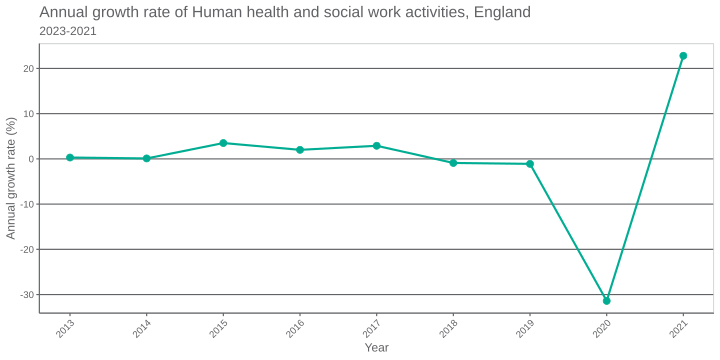
\includegraphics{./images/health_gdp_chart.svg}

\hypertarget{wrap-in-function-2}{%
\section{Wrap in function}\label{wrap-in-function-2}}

Again we should wrap this all up in a function to be called from the
\texttt{run\_analysis.R} script.

\begin{verbatim}
#' Plot data as time series
#'
#' @param data_id a string of the name of the data set to download. This is stored in config.yml as config$data_id
#' @param industry is a string of the industy we want to look at. This is stored in config.yml as config$industry
#' @param metric is a string of the metric we want to look at. This is stored in config.yml as config$metric
#' @param title is a string that will be the title of the chart
#' @param subtitle is a string that will be the subtitle of the chart
#' @param xlab is a string that is the x axis label
#' @param ylab is a string that is the y axis label
#'
#' @import DHSCtools
#' @import ggplot2
#'
#'

ts_line_chart_data <- function(data, industry, metric, title, subtitle, xlab, ylab){

  graph <- gglot2::ggplot(data = data_time_series_sorted,
         aes(Time,
             metric,
             industry)) +
    DHSCcolours::theme_dhsc() +
    geom_line(linewidth = 1) +
    geom_point(size = 3) +
    theme(legend.position="none") +
    DHSCcolours::scale_colour_dhsc_d() +
    labs(
      title = title,
      subtitle = subtitle,
      x = xlab,
      y = ylab) +
    scale_x_continuous(breaks=seq(2013,2021,1))
    
    
  #save chart
  chart_path <- paste0("./output/", metric, "_", industry, "_chart.svg")
  
  ggplot2::ggsave(chart_path,
         plot = graph,
         height = 5,
         width = 10,
         units="in",
         dpi=300)
  
  logger$info(paste0("Graph saved to: ", chart_path))
         
  return(graph)
  
}
\end{verbatim}

\bookmarksetup{startatroot}

\hypertarget{qa-documentation-toolkit}{%
\chapter{QA Documentation Toolkit}\label{qa-documentation-toolkit}}

\begin{tcolorbox}[enhanced jigsaw, arc=.35mm, colbacktitle=quarto-callout-note-color!10!white, toprule=.15mm, titlerule=0mm, opacityback=0, title=\textcolor{quarto-callout-note-color}{\faInfo}\hspace{0.5em}{Key Points}, coltitle=black, bottomrule=.15mm, colframe=quarto-callout-note-color-frame, leftrule=.75mm, breakable, opacitybacktitle=0.6, rightrule=.15mm, left=2mm, bottomtitle=1mm, toptitle=1mm, colback=white]

\begin{itemize}
\item
  Quality Assurance is essential, as described in the
  \href{https://www.gov.uk/government/publications/the-aqua-book-guidance-on-producing-quality-analysis-for-government}{AquA
  book}
\item
  The level of QA should be proportionate to the analytical work
\item
  Code needs an extra layer of QA, set out in the
  \href{https://best-practice-and-impact.github.io/qa-of-code-guidance/intro.html}{Duck
  book}
\end{itemize}

\end{tcolorbox}

Quality assurance is an essential part of all analytical work, as laid
out in the
\href{https://www.gov.uk/government/publications/the-aqua-book-guidance-on-producing-quality-analysis-for-government}{AquA
book}

This lays out the need for proportionate analytical quality assurance to
ensure that analysis and supporting model, data and assumptions are
fit-for-purpose. The main QA principles should be applied to all
projects:

\begin{itemize}
\tightlist
\item
  Governance and Oversight
\item
  Documentation
\item
  Structure and Clarity
\item
  Data and Assumptions
\item
  Validation - Am I building the right product?
\item
  Verification - Am I building the product right?
\end{itemize}

For more information on QA in general, please refer to the AQuA book, or
departmental AQA training (e.g.~Analyst Academy sessions).

\hypertarget{code-qa}{%
\section{Code QA}\label{code-qa}}

For projects using code and using this RAP template, you will need a
different approach to the verification aspect of QA. The other QA is
still required for \textbf{all} projects to a proportionate level.

Best practice guidance for code QA can be found in the `Duck book':
\href{https://best-practice-and-impact.github.io/qa-of-code-guidance/intro.html}{Quality
assurance of code for analysis and research}

This includes a QA checklist that this guidance is based on.

\hypertarget{qa-documentation-toolkit-1}{%
\section{QA documentation toolkit}\label{qa-documentation-toolkit-1}}

The QA documentation toolkit has been developed from the guidance in the
Duck book to provide a template for determining the appropriate level of
QA for your project and checking the aspects to be completed.

\hypertarget{summary-page}{%
\subsection{Summary Page}\label{summary-page}}

The first page is a summary page that describes the different levels of
the QA template to use dependent on risk.

There are two risk dimensions:

\begin{itemize}
\tightlist
\item
  Code complexity (more complex code requires a higher level of QA)
\item
  Centrality to decision making processes (if an error in the analysis
  will have significant impacts on patient care, or financial, legal,
  reputational or operational impacts, it will require a higher level of
  QA)
\end{itemize}

There are three levels of QA described:

\begin{itemize}
\tightlist
\item
  Light-touch QA, e.g.~for ad-hoc one off analysis or data request.

  \begin{itemize}
  \tightlist
  \item
    Code is straightforward with few modules and functions
  \item
    Code will not be used for key decision making or frequently relied
    on to provide results
  \end{itemize}
\item
  Moderate QA e.g.~for submissions, internal dashboards or briefings

  \begin{itemize}
  \tightlist
  \item
    Moderately complex code involving multiple scripts and dependencies
  \item
    Code may be used to inform key decision making but there is low to
    moderate residual risk associated with its use
  \end{itemize}
\item
  Developed QA e.g.~for Public facing dashboards, published statisticsm
  ministerial dashboards or Impact Assessments

  \begin{itemize}
  \tightlist
  \item
    Highly complex code with a large number of scripts and dependencies
  \item
    Code will be used for key decision making or frequently relied on to
    provide results
  \end{itemize}
\end{itemize}

\begin{figure}

{\centering 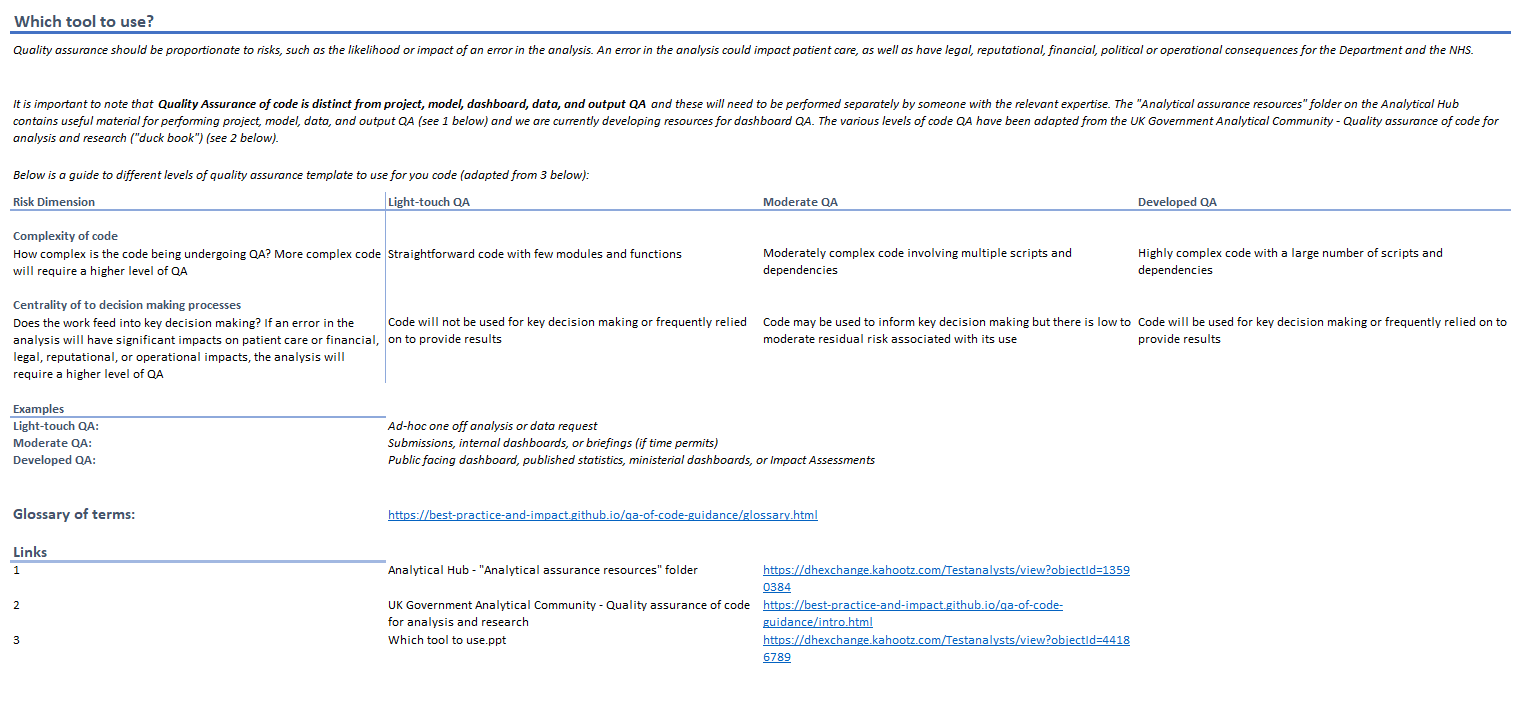
\includegraphics{./images/Screenshot QA toolkit summary page.png}

}

\caption{Screenshot of the summary page of the QA toolkit}

\end{figure}

\hypertarget{code-summary-page}{%
\subsection{Code Summary Page}\label{code-summary-page}}

This page of the toolkit requires you to record details of the code such
as it's location, the QA requestor and the responsible analyst.

\begin{figure}

{\centering 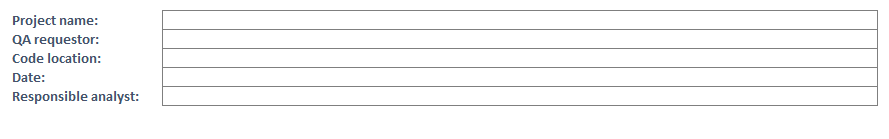
\includegraphics{./images/Screenshot QA toolkit code summary page.png}

}

\caption{Screenshot of the code summary page of the QA toolkit}

\end{figure}

\hypertarget{checklist---code-qa-page}{%
\subsection{Checklist - Code QA Page}\label{checklist---code-qa-page}}

The QA checklist is found on the final page of the toolkit.\\
On the left hand side it has a list of QA checks to be completed. These
are split into 8 sections:

\begin{enumerate}
\def\labelenumi{\arabic{enumi}.}
\tightlist
\item
  Code follows best practice and includes logging
\item
  Code is modularised/packaged, to aid maintainability, and has a clear
  structure\\
\item
  Code is documented and well commented (explaining the why not what)
  and these are maintained/accessible
\item
  README and project files present and complete
\item
  Code is under version control and CI leveraged if appropriate
\item
  Configuration and data management are in place
\item
  Code is reviews and signed-off with unit testing used where
  appropriate
\item
  All dependencies and environment settings are documented and minimised
\end{enumerate}

If you are familiar enough with what needs to be covered under these
headings, it may not be necessary to fill out every line of the
checklist. The level of detail you provide as QAer should be
proportionate to the level of QA required e.g.~light touch QA of an ad
hoc piece of analysis may only require a brief summary under each of the
8 headings above.

The checklist asks you to complete the following information:

\begin{itemize}
\tightlist
\item
  Contact of person who performed the check
\item
  Date QA performed
\item
  Current status (e.g.~are there any issues?)
\item
  Work to be done to improve assurance or quality (actions suggested by
  code QA reviewer)
\item
  Date improvements/minor fixes implemented and re-checked (major
  changes should require new QA)
\end{itemize}

On the right hand side the checklist shows which checks must be
completed dependent on the level of QA needed (identified from the
information on the summary page): All (levels), Moderate \& Developed
(levels only) or Developed (level only).

\begin{figure}

{\centering 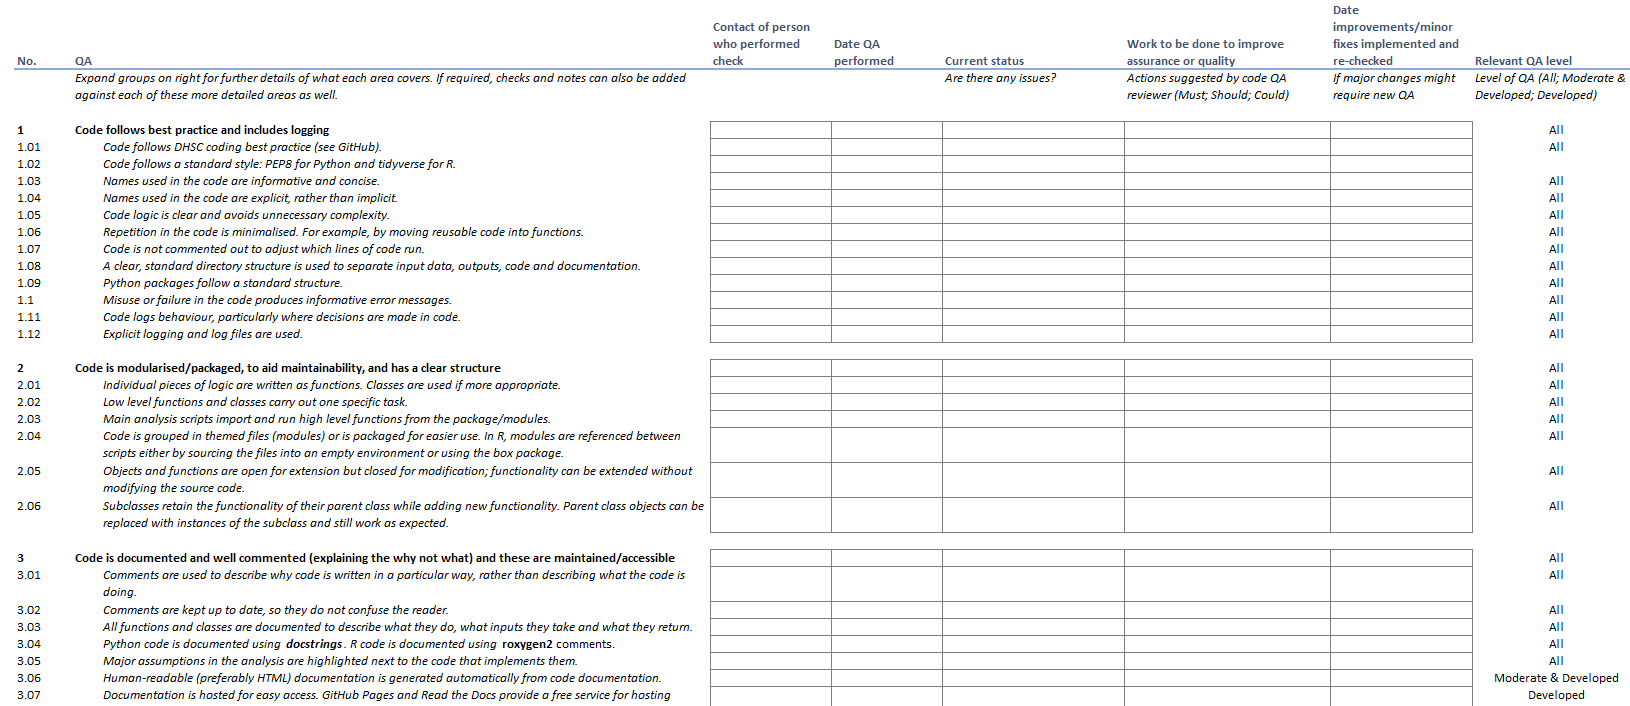
\includegraphics{./images/Screenshot QA toolkit checklist page.png}

}

\caption{Screenshot of the QA checklist page of the QA toolkit}

\end{figure}

\bookmarksetup{startatroot}

\hypertarget{example-scripts}{%
\chapter{Example scripts}\label{example-scripts}}

\bookmarksetup{startatroot}

\hypertarget{main.r}{%
\chapter{main.r}\label{main.r}}

\begin{Shaded}
\begin{Highlighting}[]
\CommentTok{\# install packages if needed}

\ControlFlowTok{if}\NormalTok{ (}\SpecialCharTok{!}\FunctionTok{requireNamespace}\NormalTok{(}\StringTok{"librarian"}\NormalTok{)) }\FunctionTok{install.packages}\NormalTok{(}\StringTok{"librarian"}\NormalTok{, }\AttributeTok{quiet =} \ConstantTok{TRUE}\NormalTok{)}

  \FunctionTok{suppressWarnings}\NormalTok{(}
\NormalTok{    librarian}\SpecialCharTok{::}\FunctionTok{shelf}\NormalTok{(}
\NormalTok{      DataS}\SpecialCharTok{{-}}\NormalTok{DHSC}\SpecialCharTok{/}\NormalTok{DHSClogger,}
\NormalTok{      ggplot2,}
\NormalTok{      httr,}
\NormalTok{      jsonlite,}
\NormalTok{      dplyr,}
\NormalTok{      readr,}
\NormalTok{      DHSCcolours,}
      \AttributeTok{quiet =} \ConstantTok{TRUE}\NormalTok{))}

\CommentTok{\# Setup logging}
\NormalTok{logger }\OtherTok{\textless{}{-}}\NormalTok{ DHSClogger}\SpecialCharTok{::}\FunctionTok{get\_dhsc\_logger}\NormalTok{()}

\CommentTok{\# set threshold of console log to information and above}
\NormalTok{logger}\SpecialCharTok{$}\FunctionTok{set\_threshold}\NormalTok{(}\StringTok{"log.console"}\NormalTok{, }\StringTok{"INFO"}\NormalTok{)}

\CommentTok{\# read in config.yml}
\NormalTok{config }\OtherTok{\textless{}{-}}\NormalTok{ yaml}\SpecialCharTok{::}\FunctionTok{read\_yaml}\NormalTok{(}
    \FunctionTok{file.path}\NormalTok{(}\StringTok{"input"}\NormalTok{, }\StringTok{"config.yml"}\NormalTok{)}
\NormalTok{  )}

\CommentTok{\#run analysis}
\FunctionTok{source}\NormalTok{(}\StringTok{"r/run\_analysis.r"}\NormalTok{)}
\FunctionTok{run\_analysis}\NormalTok{()}
\end{Highlighting}
\end{Shaded}

\bookmarksetup{startatroot}

\hypertarget{run_analysis.r}{%
\chapter{run\_analysis.r}\label{run_analysis.r}}

\begin{Shaded}
\begin{Highlighting}[]
\CommentTok{\#read in your analysis functions}
\FunctionTok{source}\NormalTok{(}\StringTok{"r/ingest\_data.r"}\NormalTok{)}
\FunctionTok{source}\NormalTok{(}\StringTok{"r/process\_data.r"}\NormalTok{)}
\FunctionTok{source}\NormalTok{(}\StringTok{"r/process\_data.r"}\NormalTok{)}

\CommentTok{\#read in data}
\FunctionTok{download\_data\_from\_ons}\NormalTok{(}\AttributeTok{data\_id =}\NormalTok{ config}\SpecialCharTok{$}\NormalTok{data\_id)}

\CommentTok{\#process data}
\NormalTok{ons\_data }\OtherTok{\textless{}{-}} \FunctionTok{process\_data}\NormalTok{(}\AttributeTok{data\_id =}\NormalTok{ config}\SpecialCharTok{$}\NormalTok{data\_id, }
                     \AttributeTok{industry =}\NormalTok{ config}\SpecialCharTok{$}\NormalTok{industry,}
                     \AttributeTok{geography =}\NormalTok{ config}\SpecialCharTok{$}\NormalTok{geography,}
                     \AttributeTok{metric =}\NormalTok{ config}\SpecialCharTok{$}\NormalTok{metric)}

\CommentTok{\#plot data}
\NormalTok{chart }\OtherTok{\textless{}{-}} \FunctionTok{ts\_line\_chart\_data}\NormalTok{(}\AttributeTok{data =}\NormalTok{ ons\_data, }
                            \AttributeTok{industry =}\NormalTok{ config}\SpecialCharTok{$}\NormalTok{industry,}
                            \AttributeTok{metric =}\NormalTok{ config}\SpecialCharTok{$}\NormalTok{metric, }
                            \AttributeTok{title =}\NormalTok{ config}\SpecialCharTok{$}\NormalTok{chart\_title, }
                            \AttributeTok{subtitle =}\NormalTok{ config}\SpecialCharTok{$}\NormalTok{subchart\_title, }
                            \AttributeTok{xlab =}\NormalTok{ config}\SpecialCharTok{$}\NormalTok{xlab, }
                            \AttributeTok{ylab =}\NormalTok{ config}\SpecialCharTok{$}\NormalTok{ylab)}

\NormalTok{chart}
\end{Highlighting}
\end{Shaded}

\bookmarksetup{startatroot}

\hypertarget{config.yml}{%
\chapter{config.yml}\label{config.yml}}

\begin{verbatim}
# see https://cran.r-project.org/web/packages/ymlthis/vignettes/yaml-overview.html
# for details of writing yaml files

data_dictionary_url: "https://api.beta.ons.gov.uk/v1/datasets"
data_id: "regional-gdp-by-year"
input_dir: ./input
output_dir: ./output
industry : "Q: Human health and social work activities"
geography : "England"
metric : "Annual growth rate"
title : "Annual growth rate of Human health and social work activities, England"
subtitle : "2013 to 2021"
xlab : "Year"
ylab : "Annual growth rate (%)"
\end{verbatim}

\bookmarksetup{startatroot}

\hypertarget{ingest_data.r}{%
\chapter{ingest\_data.r}\label{ingest_data.r}}

\begin{Shaded}
\begin{Highlighting}[]
\CommentTok{\#\textquotesingle{} Downloads a csv from the ONS API, and saves to input folder}
\CommentTok{\#\textquotesingle{}}
\CommentTok{\#\textquotesingle{} @param data\_dictionary\_url}
\CommentTok{\#\textquotesingle{} @param data\_id a string of the name of the data set to download. This is stored in config.yml as config$data\_id}
\CommentTok{\#\textquotesingle{}}
\CommentTok{\#\textquotesingle{} @import dplyr}
\CommentTok{\#\textquotesingle{} @import httr}
\CommentTok{\#\textquotesingle{} @import jsonlite}
\CommentTok{\#\textquotesingle{} @import logger}
\CommentTok{\#\textquotesingle{} @import readr}
\CommentTok{\#\textquotesingle{}}
\CommentTok{\#\textquotesingle{}}
\NormalTok{download\_data\_from\_ons }\OtherTok{\textless{}{-}} \ControlFlowTok{function}\NormalTok{(data\_dictionary\_url, data\_id)\{}
\CommentTok{\# request the data dictionary from the ONS api endpoint}
\NormalTok{  path }\OtherTok{\textless{}{-}}\NormalTok{ config}\SpecialCharTok{$}\NormalTok{data\_dictionary\_url}
\NormalTok{  request }\OtherTok{\textless{}{-}}\NormalTok{ httr}\SpecialCharTok{::}\FunctionTok{GET}\NormalTok{(}\AttributeTok{url =}\NormalTok{ path)}
\NormalTok{  content }\OtherTok{\textless{}{-}} \FunctionTok{rawToChar}\NormalTok{(request}\SpecialCharTok{$}\NormalTok{content)}
\NormalTok{  content\_flat }\OtherTok{\textless{}{-}}\NormalTok{ jsonlite}\SpecialCharTok{::}\FunctionTok{fromJSON}\NormalTok{(content, }\AttributeTok{flatten =} \ConstantTok{TRUE}\NormalTok{) }
  
\NormalTok{  logger}\SpecialCharTok{$}\FunctionTok{info}\NormalTok{(}\FunctionTok{paste0}\NormalTok{(}\StringTok{"Response recieved from: "}\NormalTok{, path))}
          
\CommentTok{\# create a dataframe with the downloaded data dictionary to what data is available}
\NormalTok{  df }\OtherTok{\textless{}{-}} \FunctionTok{data.frame}\NormalTok{(}\AttributeTok{id =}\NormalTok{ content\_flat}\SpecialCharTok{$}\NormalTok{items}\SpecialCharTok{$}\NormalTok{id,}
                   \AttributeTok{title =}\NormalTok{ content\_flat}\SpecialCharTok{$}\NormalTok{items}\SpecialCharTok{$}\NormalTok{title,}
                   \AttributeTok{release\_frequency =}\NormalTok{ content\_flat}\SpecialCharTok{$}\NormalTok{items}\SpecialCharTok{$}\NormalTok{release\_frequency,}
                   \AttributeTok{next\_release =}\NormalTok{ content\_flat}\SpecialCharTok{$}\NormalTok{items}\SpecialCharTok{$}\NormalTok{next\_release,}
                   \AttributeTok{description =}\NormalTok{ content\_flat}\SpecialCharTok{$}\NormalTok{items}\SpecialCharTok{$}\NormalTok{description,}
                   \AttributeTok{links\_latest\_versions =}\NormalTok{ content\_flat}\SpecialCharTok{$}\NormalTok{items}\SpecialCharTok{$}\NormalTok{links.latest\_version.href,}
                   \AttributeTok{links\_self\_href=}\NormalTok{ content\_flat}\SpecialCharTok{$}\NormalTok{items}\SpecialCharTok{$}\NormalTok{links.self.href,}
                   \AttributeTok{qmi\_href=}\NormalTok{ content\_flat}\SpecialCharTok{$}\NormalTok{items}\SpecialCharTok{$}\NormalTok{qmi.href)}
      
\NormalTok{  file\_latest\_version }\OtherTok{\textless{}{-}}\NormalTok{ df }\SpecialCharTok{\%\textgreater{}\%}
\NormalTok{   dplyr}\SpecialCharTok{::}\FunctionTok{filter}\NormalTok{(id }\SpecialCharTok{==}\NormalTok{ data\_id) }\SpecialCharTok{\%\textgreater{}\%}
\NormalTok{   dplyr}\SpecialCharTok{::}\FunctionTok{select}\NormalTok{(links\_latest\_versions) }\SpecialCharTok{\%\textgreater{}\%}
\NormalTok{   dplyr}\SpecialCharTok{::}\FunctionTok{pull}\NormalTok{()}
      
\CommentTok{\# Using the links\_latest\_versions we can get the meta data for the latest file}
\CommentTok{\# and this meta data includes the url for the latest file in either csv or xlsx}
\CommentTok{\# format. We choose .csv here. Extract it from downloads$csv$href}
      
\NormalTok{ request }\OtherTok{\textless{}{-}}\NormalTok{ httr}\SpecialCharTok{::}\FunctionTok{GET}\NormalTok{(}\AttributeTok{url =}\NormalTok{ file\_latest\_version)}
        
\NormalTok{ logger}\SpecialCharTok{$}\FunctionTok{info}\NormalTok{(}\FunctionTok{paste0}\NormalTok{(}\StringTok{"Response recieved from: "}\NormalTok{, file\_latest\_version))}
       
\NormalTok{ content }\OtherTok{\textless{}{-}} \FunctionTok{rawToChar}\NormalTok{(request}\SpecialCharTok{$}\NormalTok{content)}
\NormalTok{ content\_flat }\OtherTok{\textless{}{-}}\NormalTok{ jsonlite}\SpecialCharTok{::}\FunctionTok{fromJSON}\NormalTok{(content, }\AttributeTok{flatten=}\ConstantTok{TRUE}\NormalTok{)}
\NormalTok{ file\_url }\OtherTok{\textless{}{-}}\NormalTok{ content\_flat}\SpecialCharTok{$}\NormalTok{downloads}\SpecialCharTok{$}\NormalTok{csv}\SpecialCharTok{$}\NormalTok{href}
      
      
\CommentTok{\#Read data from latest file endpoint}
\NormalTok{ df\_data }\OtherTok{\textless{}{-}}\NormalTok{ readr}\SpecialCharTok{::}\FunctionTok{read\_csv}\NormalTok{(file\_url)}
\NormalTok{ data\_filepath }\OtherTok{\textless{}{-}} \FunctionTok{paste0}\NormalTok{(config}\SpecialCharTok{$}\NormalTok{output\_dir, }\StringTok{"/"}\NormalTok{, data\_id, }\StringTok{".csv"}\NormalTok{)}
\NormalTok{ readr}\SpecialCharTok{::}\FunctionTok{write\_csv}\NormalTok{(df\_data, data\_filepath)}
\NormalTok{ logger}\SpecialCharTok{$}\FunctionTok{info}\NormalTok{(}\FunctionTok{paste0}\NormalTok{(}\StringTok{"data output to: "}\NormalTok{, data\_filepath))}
      
\NormalTok{\}}
\end{Highlighting}
\end{Shaded}

\bookmarksetup{startatroot}

\hypertarget{process_data.r}{%
\chapter{process\_data.r}\label{process_data.r}}

\begin{Shaded}
\begin{Highlighting}[]
\CommentTok{\#\textquotesingle{} Filters relevant data and sorts it}
\CommentTok{\#\textquotesingle{}}
\CommentTok{\#\textquotesingle{} @param data\_id a string of the name of the data set to download. This is stored in config.yml as config$data\_id}
\CommentTok{\#\textquotesingle{} @param industry is a string of the industy we want to look at. This is stored in config.yml as config$industry}
\CommentTok{\#\textquotesingle{} @param geography is a string of the geography we want to look at. This is stored in config.yml as config$geography}
\CommentTok{\#\textquotesingle{} @param metric is a string of the metric we want to look at. This is stored in config.yml as config$metric}
\CommentTok{\#\textquotesingle{}}
\CommentTok{\#\textquotesingle{}}
\CommentTok{\#\textquotesingle{} @import dplyr}
\CommentTok{\#\textquotesingle{} @import logger}
\CommentTok{\#\textquotesingle{} @import readr}
\CommentTok{\#\textquotesingle{}}
\CommentTok{\#\textquotesingle{}}
\NormalTok{process\_data }\OtherTok{\textless{}{-}} \ControlFlowTok{function}\NormalTok{(data\_id, industry, geography, metric)\{}

\CommentTok{\#read in data from data ingest}
      
\NormalTok{  data\_file\_path }\OtherTok{\textless{}{-}} \FunctionTok{paste0}\NormalTok{(config}\SpecialCharTok{$}\NormalTok{output\_dir, }\StringTok{"/"}\NormalTok{, data\_id, }\StringTok{".csv"}\NormalTok{)}
\NormalTok{  data }\OtherTok{\textless{}{-}}\NormalTok{ readr}\SpecialCharTok{::}\FunctionTok{read\_csv}\NormalTok{(data\_file\_path)}
  
\NormalTok{  logger}\SpecialCharTok{$}\FunctionTok{info}\NormalTok{(}\FunctionTok{paste0}\NormalTok{(}\StringTok{"Data read from: "}\NormalTok{, data\_file\_path))}
      
\NormalTok{  data\_time\_series }\OtherTok{\textless{}{-}}\NormalTok{ data }\SpecialCharTok{\%\textgreater{}\%}
\NormalTok{    dplyr}\SpecialCharTok{::}\FunctionTok{filter}\NormalTok{(}\SpecialCharTok{!}\FunctionTok{is.na}\NormalTok{(v4\_1)) }\SpecialCharTok{\%\textgreater{}\%}
\NormalTok{    dplyr}\SpecialCharTok{::}\FunctionTok{filter}\NormalTok{(UnofficialStandardIndustrialClassification }\SpecialCharTok{==}\NormalTok{ industry) }\SpecialCharTok{\%\textgreater{}\%}
\NormalTok{    dplyr}\SpecialCharTok{::}\FunctionTok{filter}\NormalTok{(Geography }\SpecialCharTok{==}\NormalTok{ geography) }\SpecialCharTok{\%\textgreater{}\%}
\NormalTok{    dplyr}\SpecialCharTok{::}\FunctionTok{filter}\NormalTok{(GrowthRate }\SpecialCharTok{==}\NormalTok{ metric)}
        
\CommentTok{\# set year as a number and sort by}
\NormalTok{  data\_time\_series\_sorted }\OtherTok{\textless{}{-}}\NormalTok{ data\_time\_series }\SpecialCharTok{\%\textgreater{}\%}
\NormalTok{    dplyr}\SpecialCharTok{::}\FunctionTok{mutate}\NormalTok{(}\AttributeTok{Time =} \FunctionTok{as.numeric}\NormalTok{(Time)) }\SpecialCharTok{\%\textgreater{}\%}
\NormalTok{    dplyr}\SpecialCharTok{::}\FunctionTok{arrange}\NormalTok{(Time)}
        
\CommentTok{\# save data to csv}
\NormalTok{  output\_file\_name }\OtherTok{\textless{}{-}} \FunctionTok{paste0}\NormalTok{(}\StringTok{"output/"}\NormalTok{, data\_id, }\StringTok{"\_"}\NormalTok{, industry, }\StringTok{"\_"}\NormalTok{, metric, }\StringTok{"\_time\_series\_sorted.csv"}\NormalTok{)}
      
\NormalTok{  readr}\SpecialCharTok{::}\FunctionTok{write\_csv}\NormalTok{(}
\NormalTok{    data\_time\_series\_sorted,}
    \AttributeTok{file =}\NormalTok{ output\_file\_name)}
        
\NormalTok{  logger}\SpecialCharTok{$}\FunctionTok{info}\NormalTok{(}\FunctionTok{paste0}\NormalTok{(}\StringTok{"processed data saved to "}\NormalTok{, output\_file\_name))}
      
  \FunctionTok{return}\NormalTok{(data\_time\_series\_sorted)}

\NormalTok{\}}
\end{Highlighting}
\end{Shaded}

\bookmarksetup{startatroot}

\hypertarget{plot_data.r}{%
\chapter{plot\_data.r}\label{plot_data.r}}

\begin{Shaded}
\begin{Highlighting}[]
\CommentTok{\#\textquotesingle{} Plot data as time series}
\CommentTok{\#\textquotesingle{}}
\CommentTok{\#\textquotesingle{} @param data\_id a string of the name of the data set to download. This is stored in config.yml as config$data\_id}
\CommentTok{\#\textquotesingle{} @param industry is a string of the industy we want to look at. This is stored in config.yml as config$industry}
\CommentTok{\#\textquotesingle{} @param metric is a string of the metric we want to look at. This is stored in config.yml as config$metric}
\CommentTok{\#\textquotesingle{} @param title is a string that will be the title of the chart}
\CommentTok{\#\textquotesingle{} @param subtitle is a string that will be the subtitle of the chart}
\CommentTok{\#\textquotesingle{} @param xlab is a string that is the x axis label}
\CommentTok{\#\textquotesingle{} @param ylab is a string that is the y axis label}
\CommentTok{\#\textquotesingle{}}
\CommentTok{\#\textquotesingle{} @import DHSCtools}
\CommentTok{\#\textquotesingle{} @import ggplot2}
\CommentTok{\#\textquotesingle{}}
\CommentTok{\#\textquotesingle{}}

\NormalTok{ts\_line\_chart\_data }\OtherTok{\textless{}{-}} \ControlFlowTok{function}\NormalTok{(data, industry, metric, title, subtitle, xlab, ylab)\{}

\NormalTok{  graph }\OtherTok{\textless{}{-}}\NormalTok{ gglot2}\SpecialCharTok{::}\FunctionTok{ggplot}\NormalTok{(}\AttributeTok{data =}\NormalTok{ data\_time\_series\_sorted,}
                          \FunctionTok{aes}\NormalTok{(Time,}
\NormalTok{                              v4\_1,}
\NormalTok{                              industry)) }\SpecialCharTok{+}
\NormalTok{    DHSCcolours}\SpecialCharTok{::}\FunctionTok{theme\_dhsc}\NormalTok{() }\SpecialCharTok{+}
    \FunctionTok{geom\_line}\NormalTok{(}\AttributeTok{linewidth =} \DecValTok{1}\NormalTok{) }\SpecialCharTok{+}
    \FunctionTok{geom\_point}\NormalTok{(}\AttributeTok{size =} \DecValTok{3}\NormalTok{) }\SpecialCharTok{+}
    \FunctionTok{theme}\NormalTok{(}\AttributeTok{legend.position=}\StringTok{"none"}\NormalTok{) }\SpecialCharTok{+}
\NormalTok{    DHSCcolours}\SpecialCharTok{::}\FunctionTok{scale\_colour\_dhsc\_d}\NormalTok{() }\SpecialCharTok{+}
    \FunctionTok{labs}\NormalTok{(}
      \AttributeTok{title =}\NormalTok{ title,}
      \AttributeTok{subtitle =}\NormalTok{ subtitle,}
      \AttributeTok{x =}\NormalTok{ xlab,}
      \AttributeTok{y =}\NormalTok{ ylab) }\SpecialCharTok{+}
    \FunctionTok{scale\_x\_continuous}\NormalTok{(}\AttributeTok{breaks=}\FunctionTok{seq}\NormalTok{(}\DecValTok{2013}\NormalTok{,}\DecValTok{2021}\NormalTok{,}\DecValTok{1}\NormalTok{))}
        
\CommentTok{\#save chart}
\NormalTok{ chart\_path }\OtherTok{\textless{}{-}} \FunctionTok{paste0}\NormalTok{(}\StringTok{"./output/"}\NormalTok{, metric, }\StringTok{"\_"}\NormalTok{, industry, }\StringTok{"\_chart.svg"}\NormalTok{)}
      
\NormalTok{ ggplot2}\SpecialCharTok{::}\FunctionTok{ggsave}\NormalTok{(chart\_path,}
                 \AttributeTok{plot =}\NormalTok{ graph,}
                 \AttributeTok{height =} \DecValTok{5}\NormalTok{,}
                 \AttributeTok{width =} \DecValTok{10}\NormalTok{,}
                 \AttributeTok{units=}\StringTok{"in"}\NormalTok{,}
                 \AttributeTok{dpi=}\DecValTok{300}\NormalTok{)}
      
\NormalTok{ logger}\SpecialCharTok{$}\FunctionTok{info}\NormalTok{(}\FunctionTok{paste0}\NormalTok{(}\StringTok{"Graph saved to: "}\NormalTok{, chart\_path))}
             
 \FunctionTok{return}\NormalTok{(graph)}
      
\NormalTok{\}}
\end{Highlighting}
\end{Shaded}



\backmatter

\end{document}
